\chapter{Analysis of platoon behavior in the Black Forest}
\label{chapter:Analysis of platoon behaviour in the Black Forest}
This chapter investigates the platoon behavior on the selected set of streets in the Black Forest region using the rule set described in Chapter \ref{chapter:A Cellular Automata Model for Platoons}. First, the simulation results for one of the streets, the Allerheiligenstraße, are presented as an example. To keep focus the results from the other streets are shown in the appendix. Then, a ranking is generated by comparing the results of the simulations of the streets. It is important to note that this analysis only considers the curvature of the road and not other factors, such as altitude differences or whether the road passes through a town.\\

To analyze the behavior of platoons on the seven selected streets, the platoon was simulated on both an empty road and a congested road, with the platoon starting at the beginning of the road and driving to the end. The number of time-steps is determined by how many steps it takes the platoon to travel the empty road from start to finish. The simulation was run for ten loops to account for standard deviation and to smooth out the effects of initialization. Congestion was simulated at a vehicle density of 0.03, which means that 3\% of the road is occupied by vehicles. This value was obtained via visualization of traffic on a 2D-pixel plot. Additionally, the $car\_share$ parameter was set to 0.95 to simulate mixed traffic. The random chance of sudden braking and aborting of lane change decisions are turned off to achieve a more predictable behavior of the vehicles in the simulation. The platoon consists of five bikers, with Biker 0 always set as the sweeper and Biker 4 as the leader at the start of the simulation. Each simulation for a street takes approximately 20 minutes to 1 hour, depending on the number of time-steps and the length of the street. The standard deviation values are obtained from the ten loops and are used to calculate the 95\% confidence interval, which is shown in all appropriate time series plots. In addition, as the simulation is run 10 times for each road, the plots show the mean of all calculated values.\\


\begin{landscape}
  \begin{figure}
    \centering
    \begin{subfigure}[b]{1.0\linewidth}
      \centering
      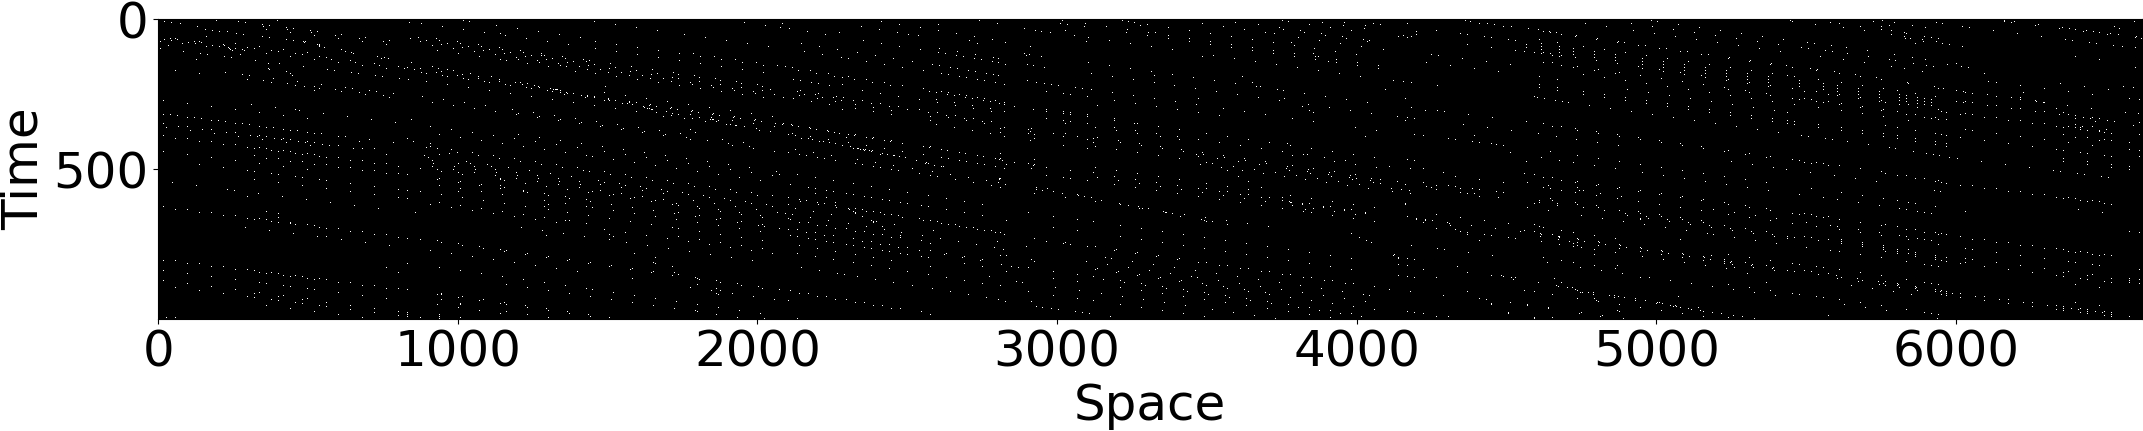
\includegraphics[width=\textwidth]{images/Allerheiligenstraße/Allerheiligenstrase_2D_left_congested.png}
      \caption{Left lane}
    \end{subfigure}
    \hfill
    \begin{subfigure}[b]{1.0\linewidth}
      \centering
      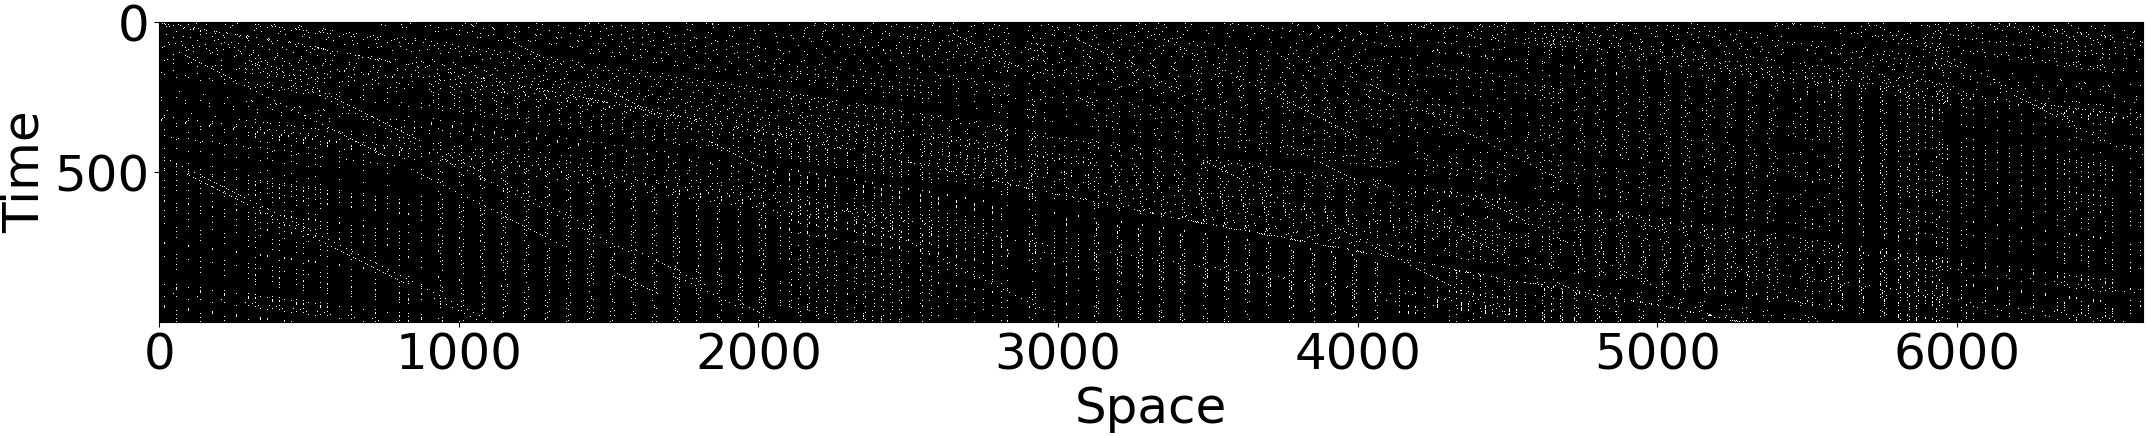
\includegraphics[width=\textwidth]{images/Allerheiligenstraße/Allerheiligenstrase_2D_right_congested.png}
      \caption{Right lane}
    \end{subfigure}
    \caption{2D-Pixel Plot for Allerheiligenstraße with a $density$ of 3\%. White dots represent a vehicle.}
    \label{fig:Allerheiligenstraße_2D}
  \end{figure}
\end{landscape}


\section{Analysis of a Platoon on Allerheiligenstraße}
\label{Analysis of a Platoon on Allerheiligenstraße}
This section provides an analysis of the platoon behavior on the Allerheiligenstraße as an example. Figure \ref{fig:Allerheiligenstraße} is used to show the Allerheiligenstraße street, and figure \ref{fig:Allerheiligenstraße_2D} is used to display the corresponding congested 2D-pixel plot of the street. It is worth noting that the vertical lines observed in the 2D pixel plot occur due to sudden changes in curvature, resulting in a steep decrease in the maximum allowed speed. As a consequence, the vehicles decrease their speed to the same value, leading to the appearance of vertical lines on the plot. Furthermore, it is important to note that these vertical lines become stronger in the absence of random sudden brakes, which are turned off in this simulation.\\

Figure \ref{fig:Allerheiligenstraße_fun_distribution} shows the fun-distribution over each time-step for the five motorcyclists on this street. The curve on the free traffic plot shows erratic but consistent behavior. This is due to the slow formation of the platoon, which takes at least about 15 time-steps for a platoon of five members to adjust, and since there are no random disturbances from traffic, the driving behavior is deterministic. The curve also shows a plateau at the beginning of the first 100 time steps, which is not the maximum possible. It does not reach the maximum because the curvature of the road is low, and the weight for speed on a road with a curvature < 400 is only 0.25 compared with higher curvatures. The highest possible peak can be found e.g. between 200 and 300 time steps of about 1.2. Additionally, the fun metric for the motorcyclists behaves poorly when road sections with big changes in curvature appear next to each other in a short distance, resulting in dips in the fun-distribution curve of the whole platoon. This is especially evident in the middle of the Allerheiligenstraße trip, as this road exhibits high curvature around the middle. One would rather expect an increase in the fun-distribution curve, but a decrease can be observed instead. As expected, the fun-distribution curve for congested traffic shows a smoother behavior and lower values in general due to the traffic, and a better correlation of the fun-distribution curve with the curvature of the road can be observed. However, this correlation may not be straightforward to see and could be incorrect.\\


\begin{figure}
\centering
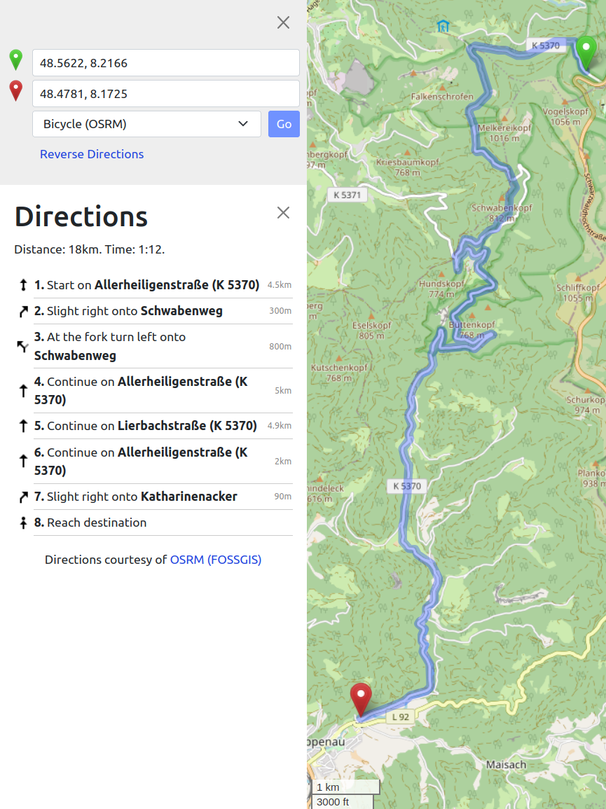
\includegraphics[width=0.7\linewidth]{images/Allerheiligenstraße/Allerheiligenstrase.png}
\caption{Allerheiligenstraße (K 5370), source: openstreetmap.org, 19.02.2023}
\label{fig:Allerheiligenstraße}
\end{figure}

\begin{figure}[h]
     \centering
     \begin{subfigure}[b]{1.0\textwidth}
         \centering
         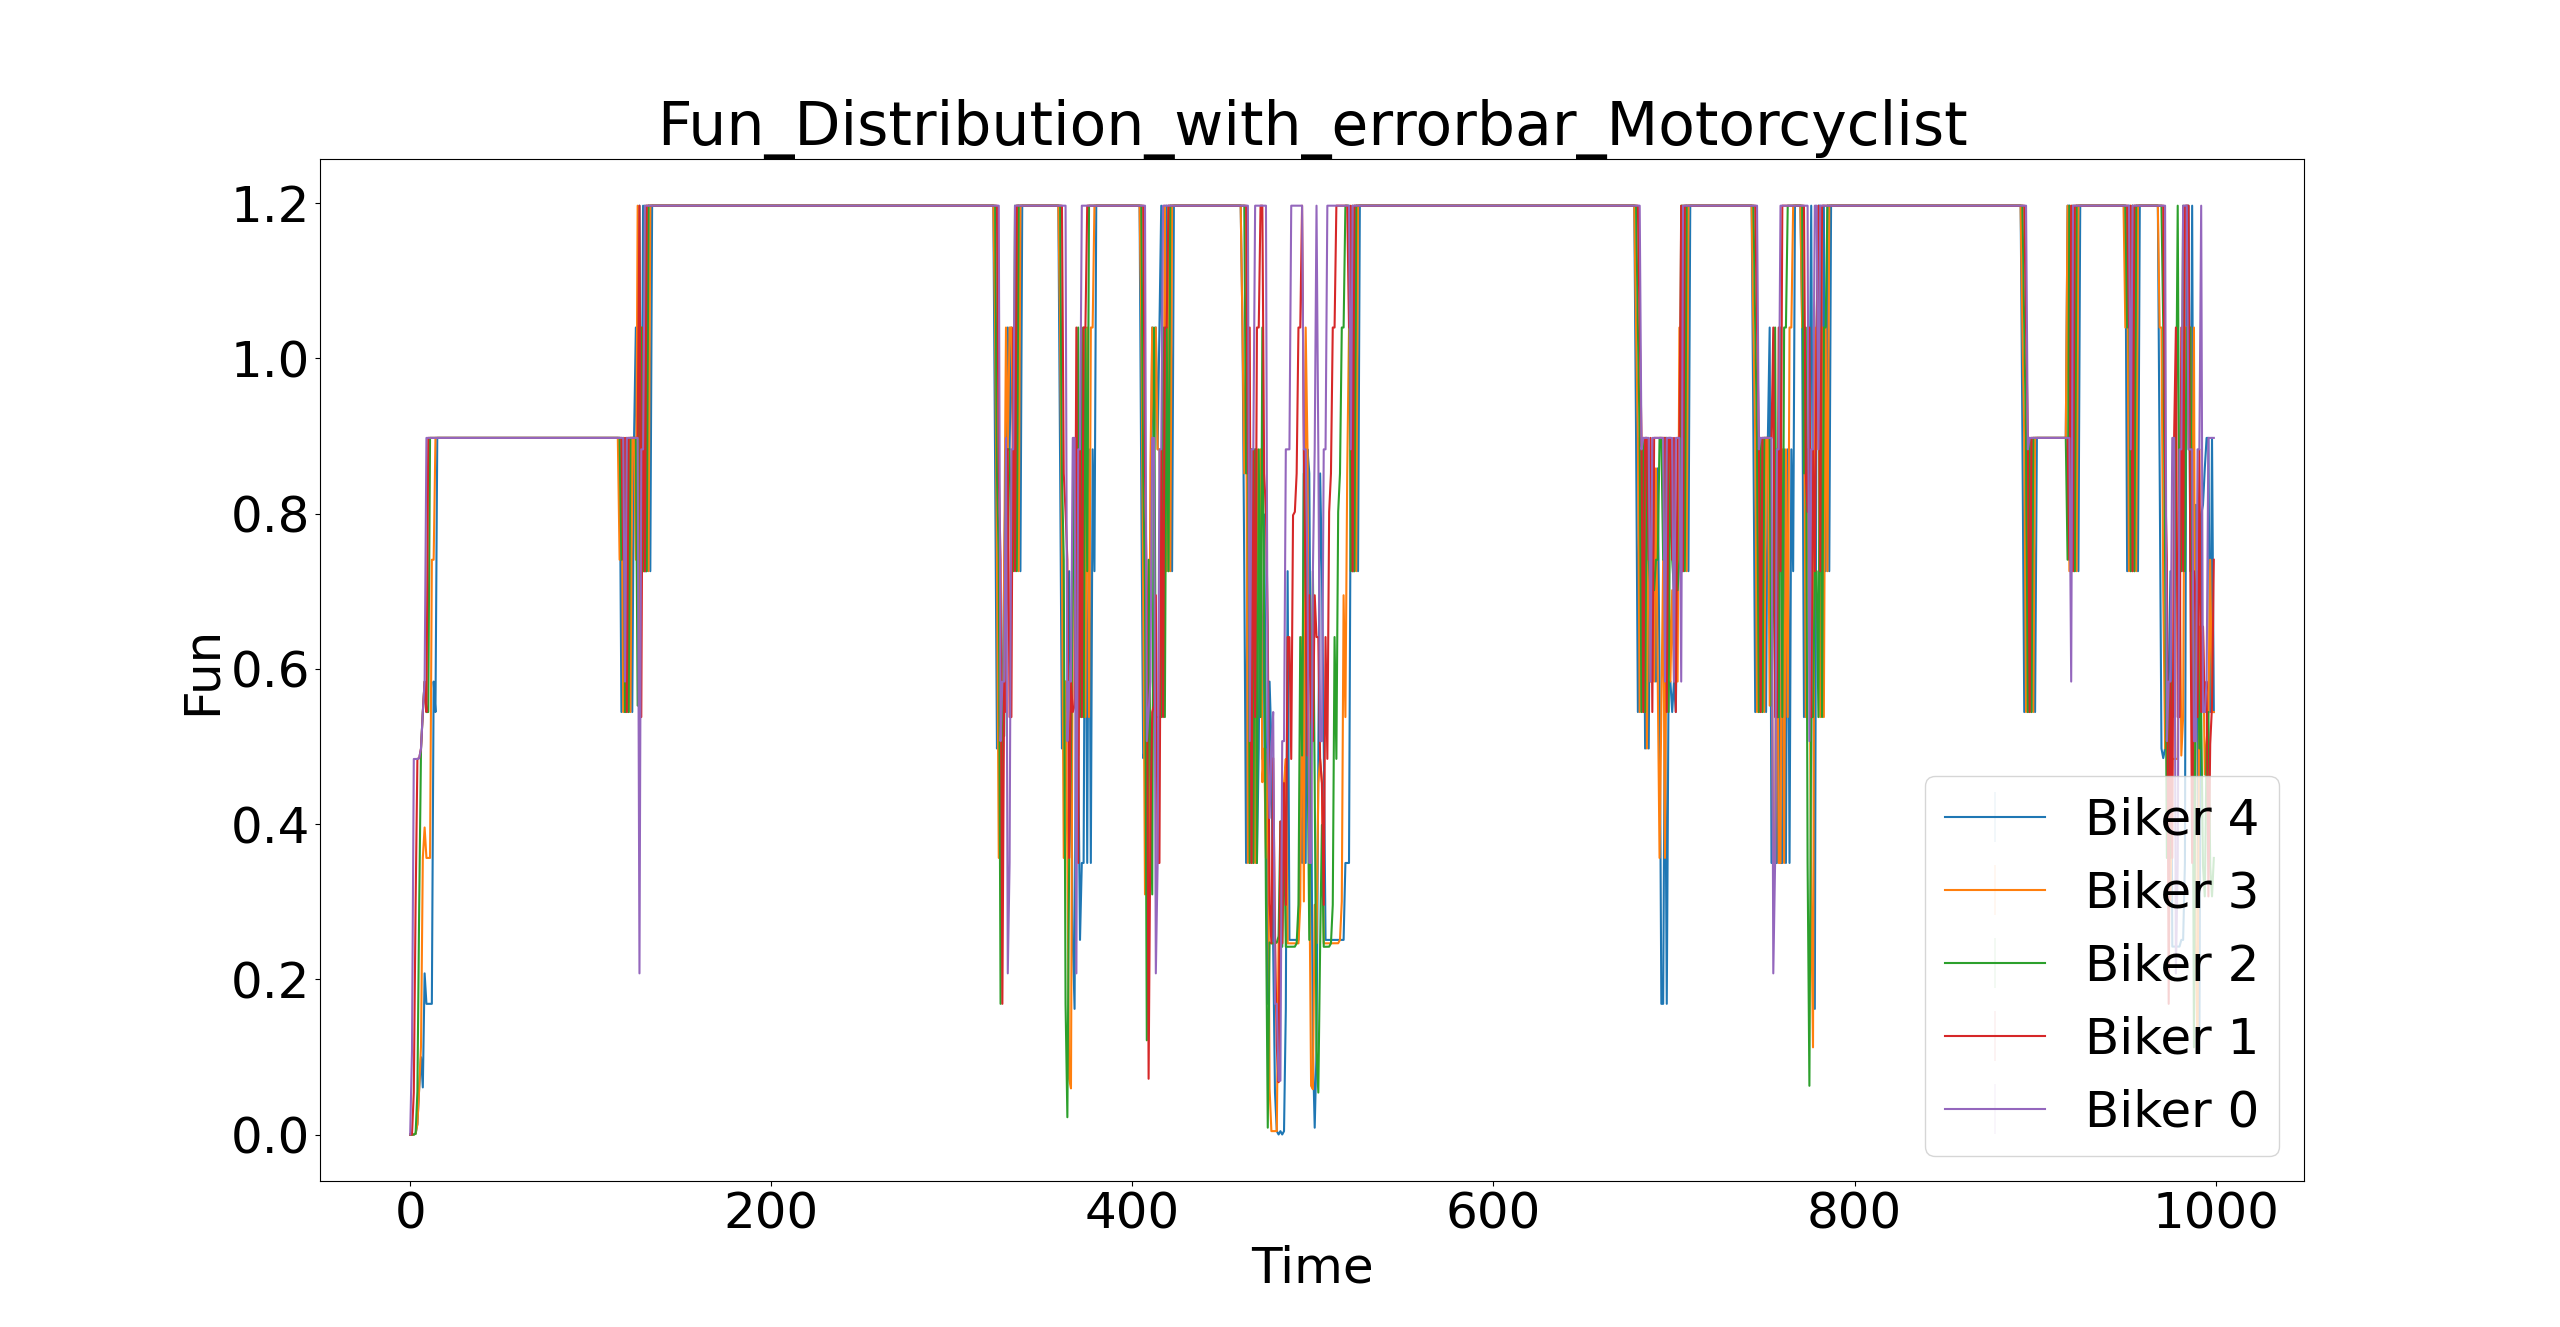
\includegraphics[width=\textwidth]{images/Allerheiligenstraße/Allerheiligenstrase_Fun_Distribution_with_errorbar_free.png}
         \caption{free traffic}
     \end{subfigure}
     \hfill
     \begin{subfigure}[b]{1.0\textwidth}
         \centering
         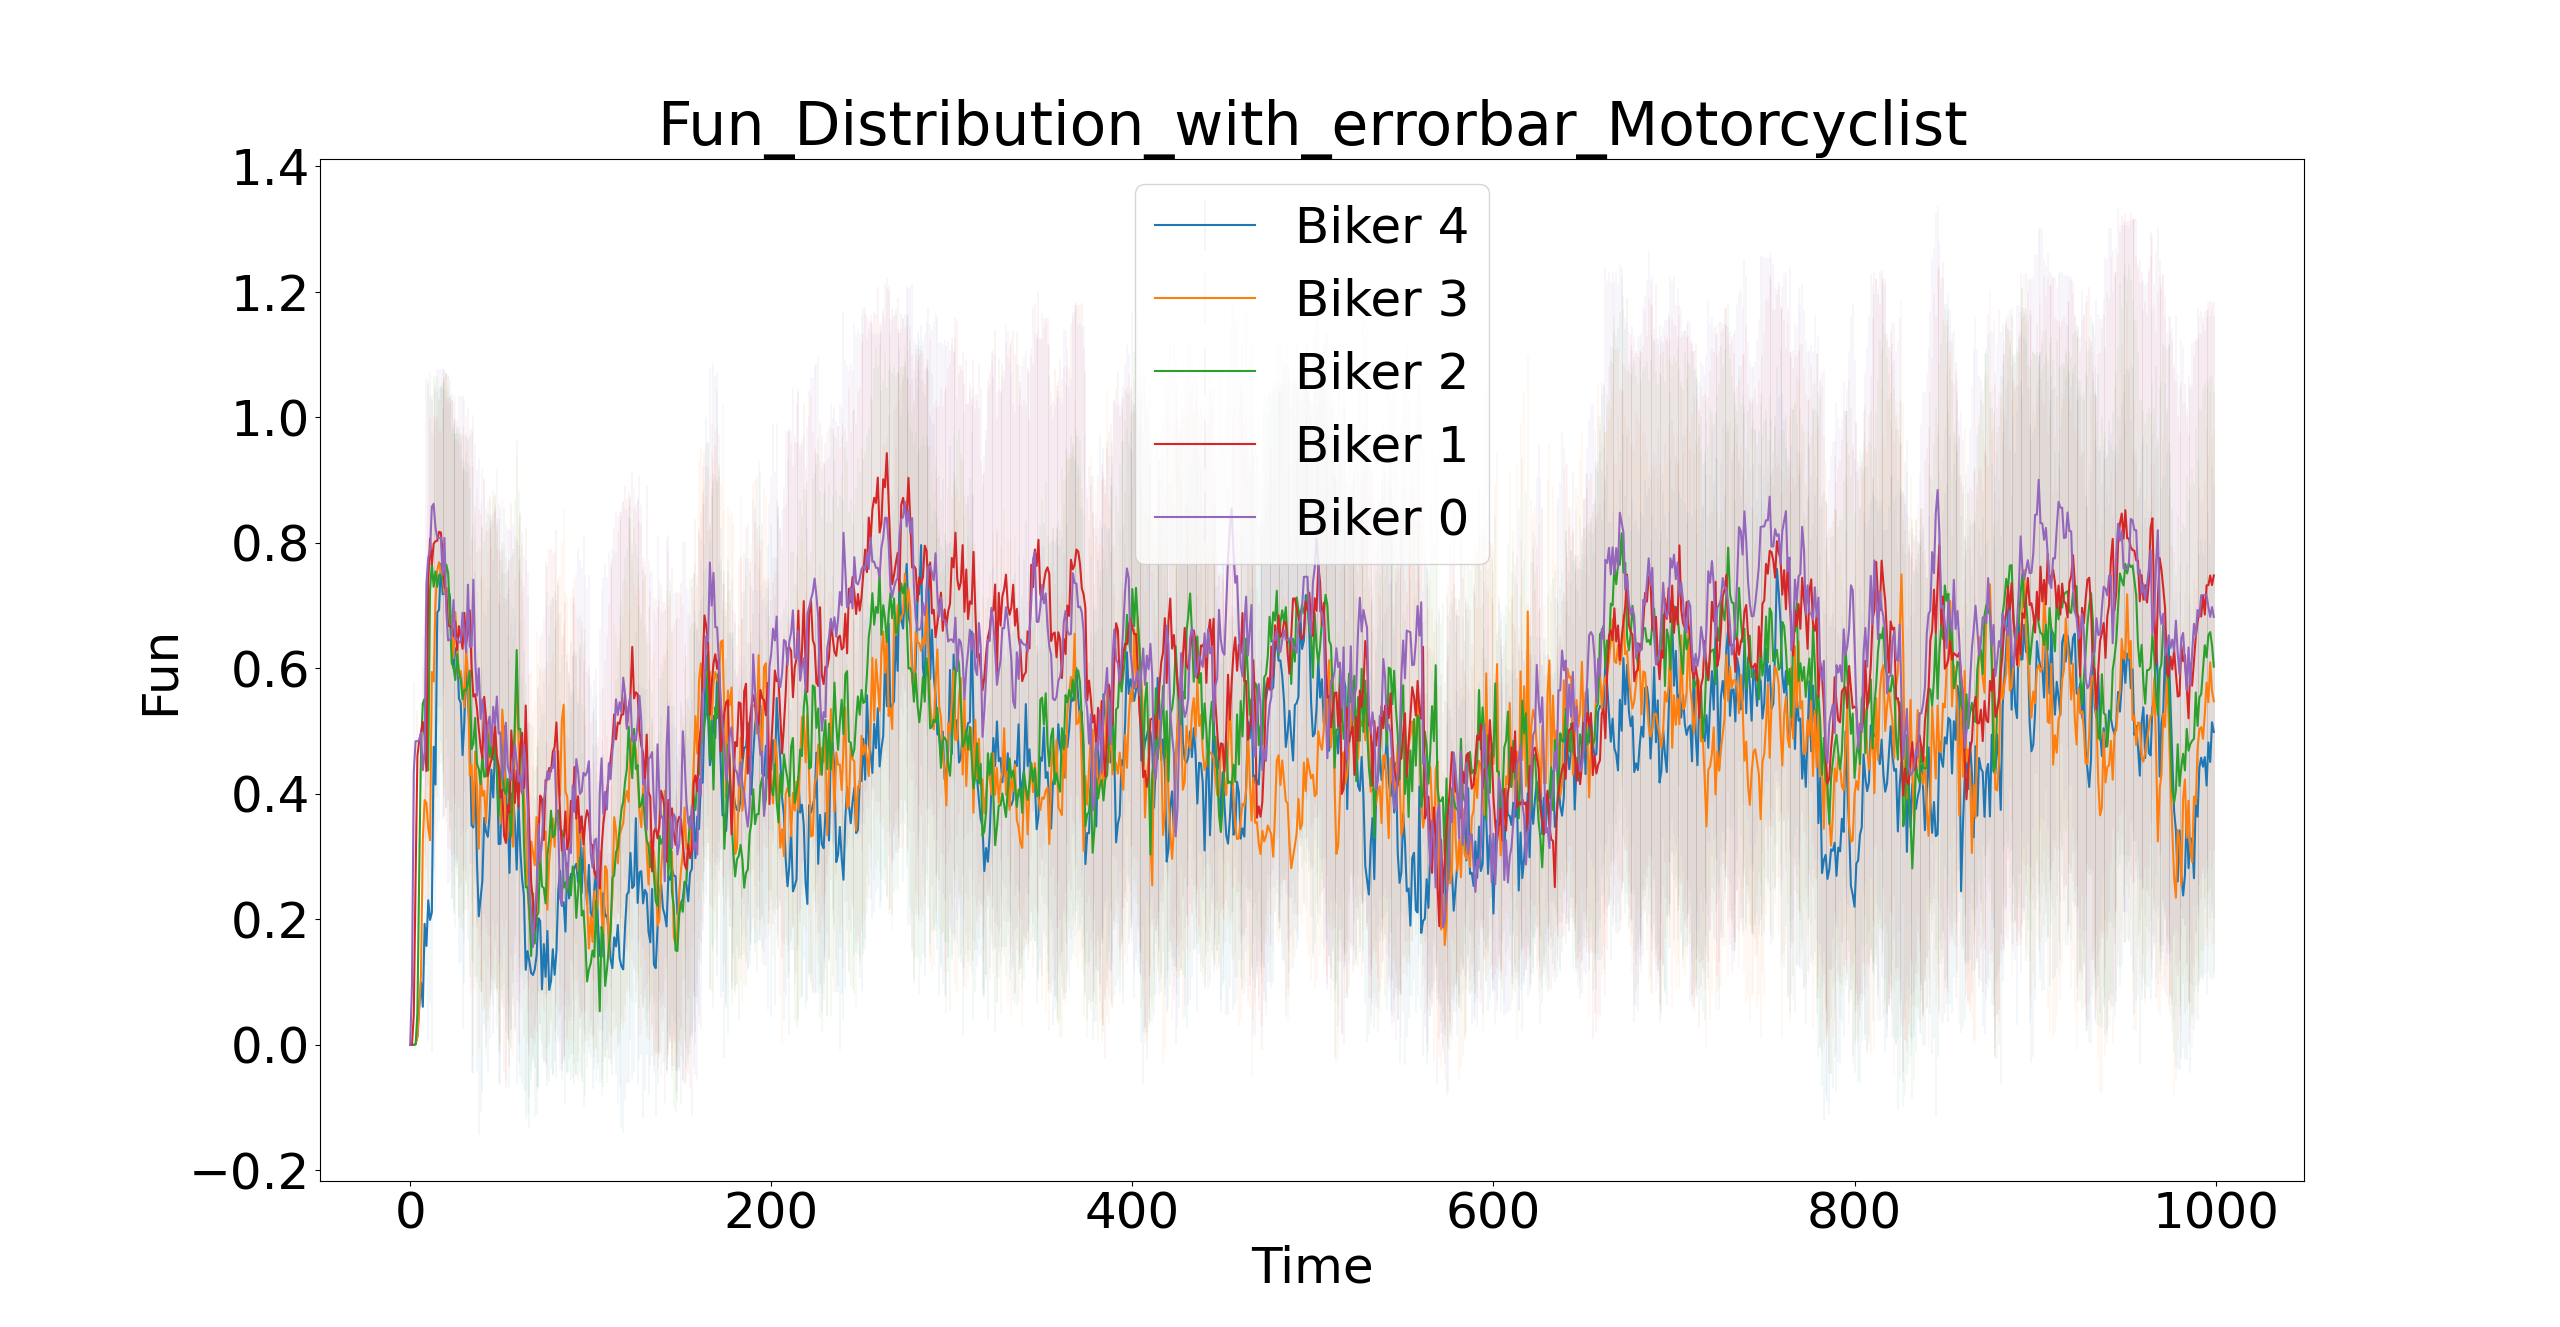
\includegraphics[width=\textwidth]{images/Allerheiligenstraße/Allerheiligenstrase_Fun_Distribution_with_errorbar_congested.png}
         \caption{congested traffic}
     \end{subfigure}
        \caption{Fun-distribution of five motorcyclists for Allerheiligenstraße}
        \label{fig:Allerheiligenstraße_fun_distribution}
\end{figure}

The mean fun-value experienced by a motorcyclist on the Allerheiligenstraße street is shown in Figure \ref{fig:Allerheiligenstraße_fun_histogram}. The histogram reveals that motorcyclists positioned at the front of the platoon experience lower fun-values during the trip, irrespective of the level of vehicle density on the street. This effect is exacerbated in congested traffic conditions. Since the platoon is modeled as a line, and the motorcyclists do not overtake each other on their own, the leader has to wait for those behind, leading to lower fun-values. Additionally, the initial leader typically remains in the lead throughout the trip, as indicated by the role distribution in Figure \ref{fig:Allerheiligenstraß_role_histogram}. The lack of any motorcyclist being lost during the simulation may be attributed to the small size of the platoon.\\

\begin{figure}
     \centering
     \begin{subfigure}[b]{1.0\textwidth}
         \centering
         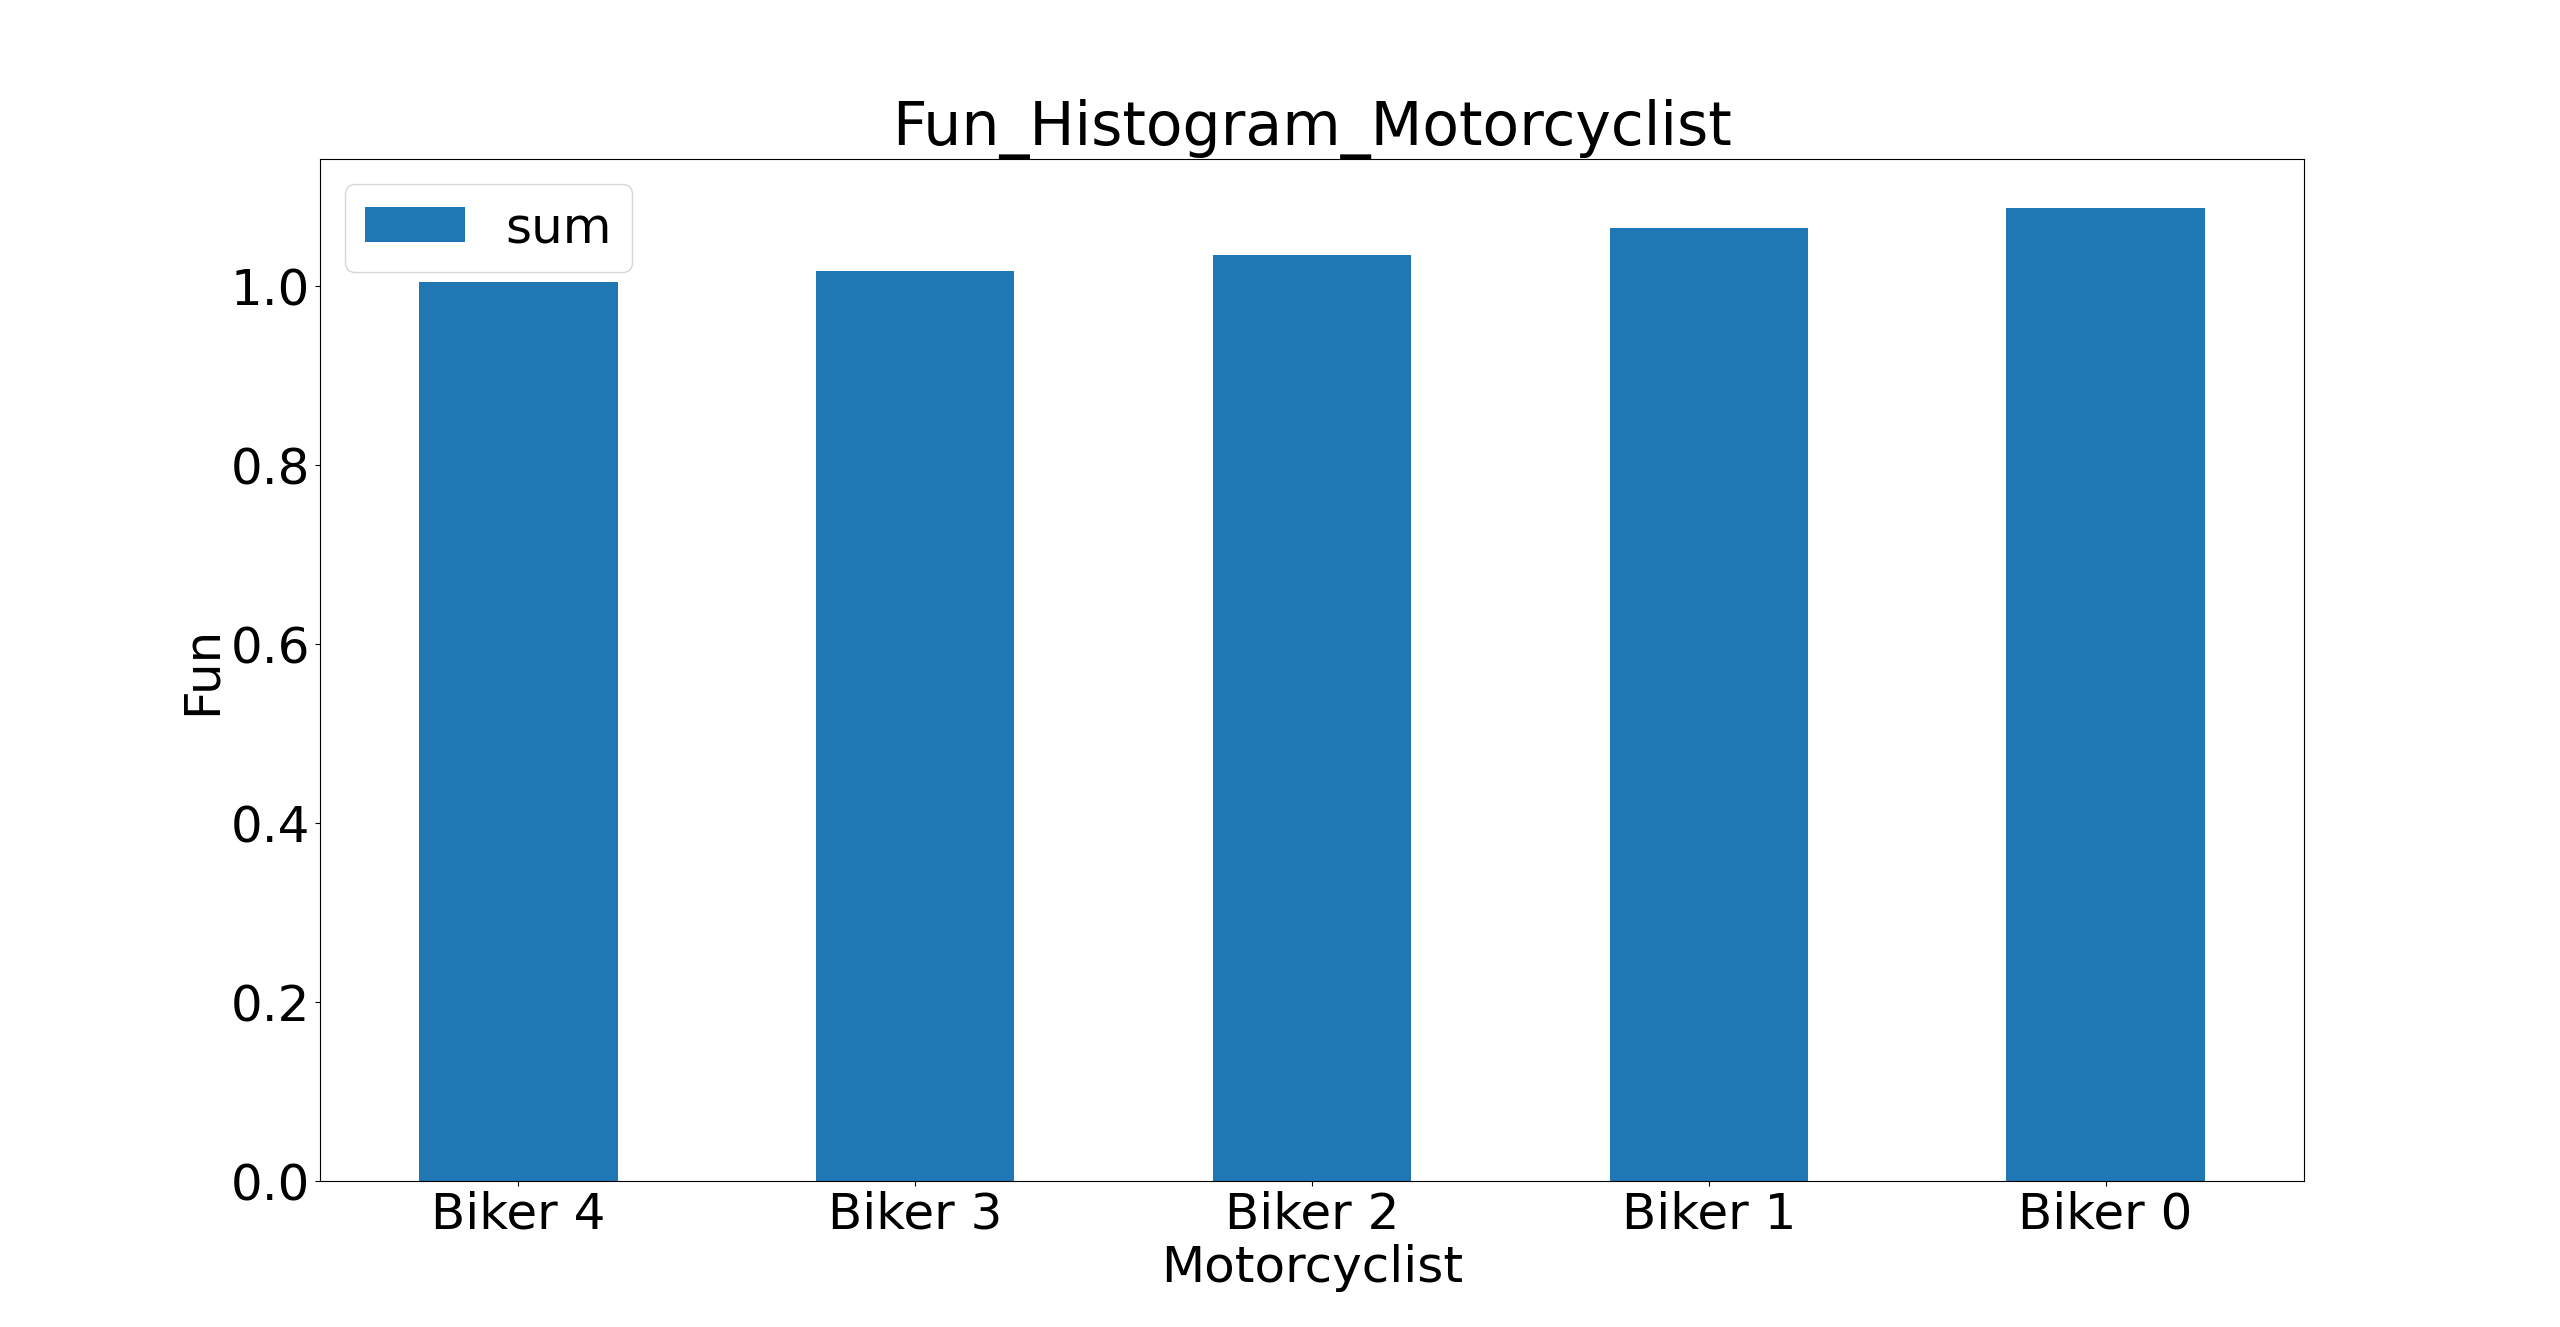
\includegraphics[width=\textwidth]{images/Allerheiligenstraße/Allerheiligenstrase_Fun_Histogram_free.png}
         \caption{free traffic}
     \end{subfigure}
     \hfill
     \begin{subfigure}[b]{1.0\textwidth}
         \centering
         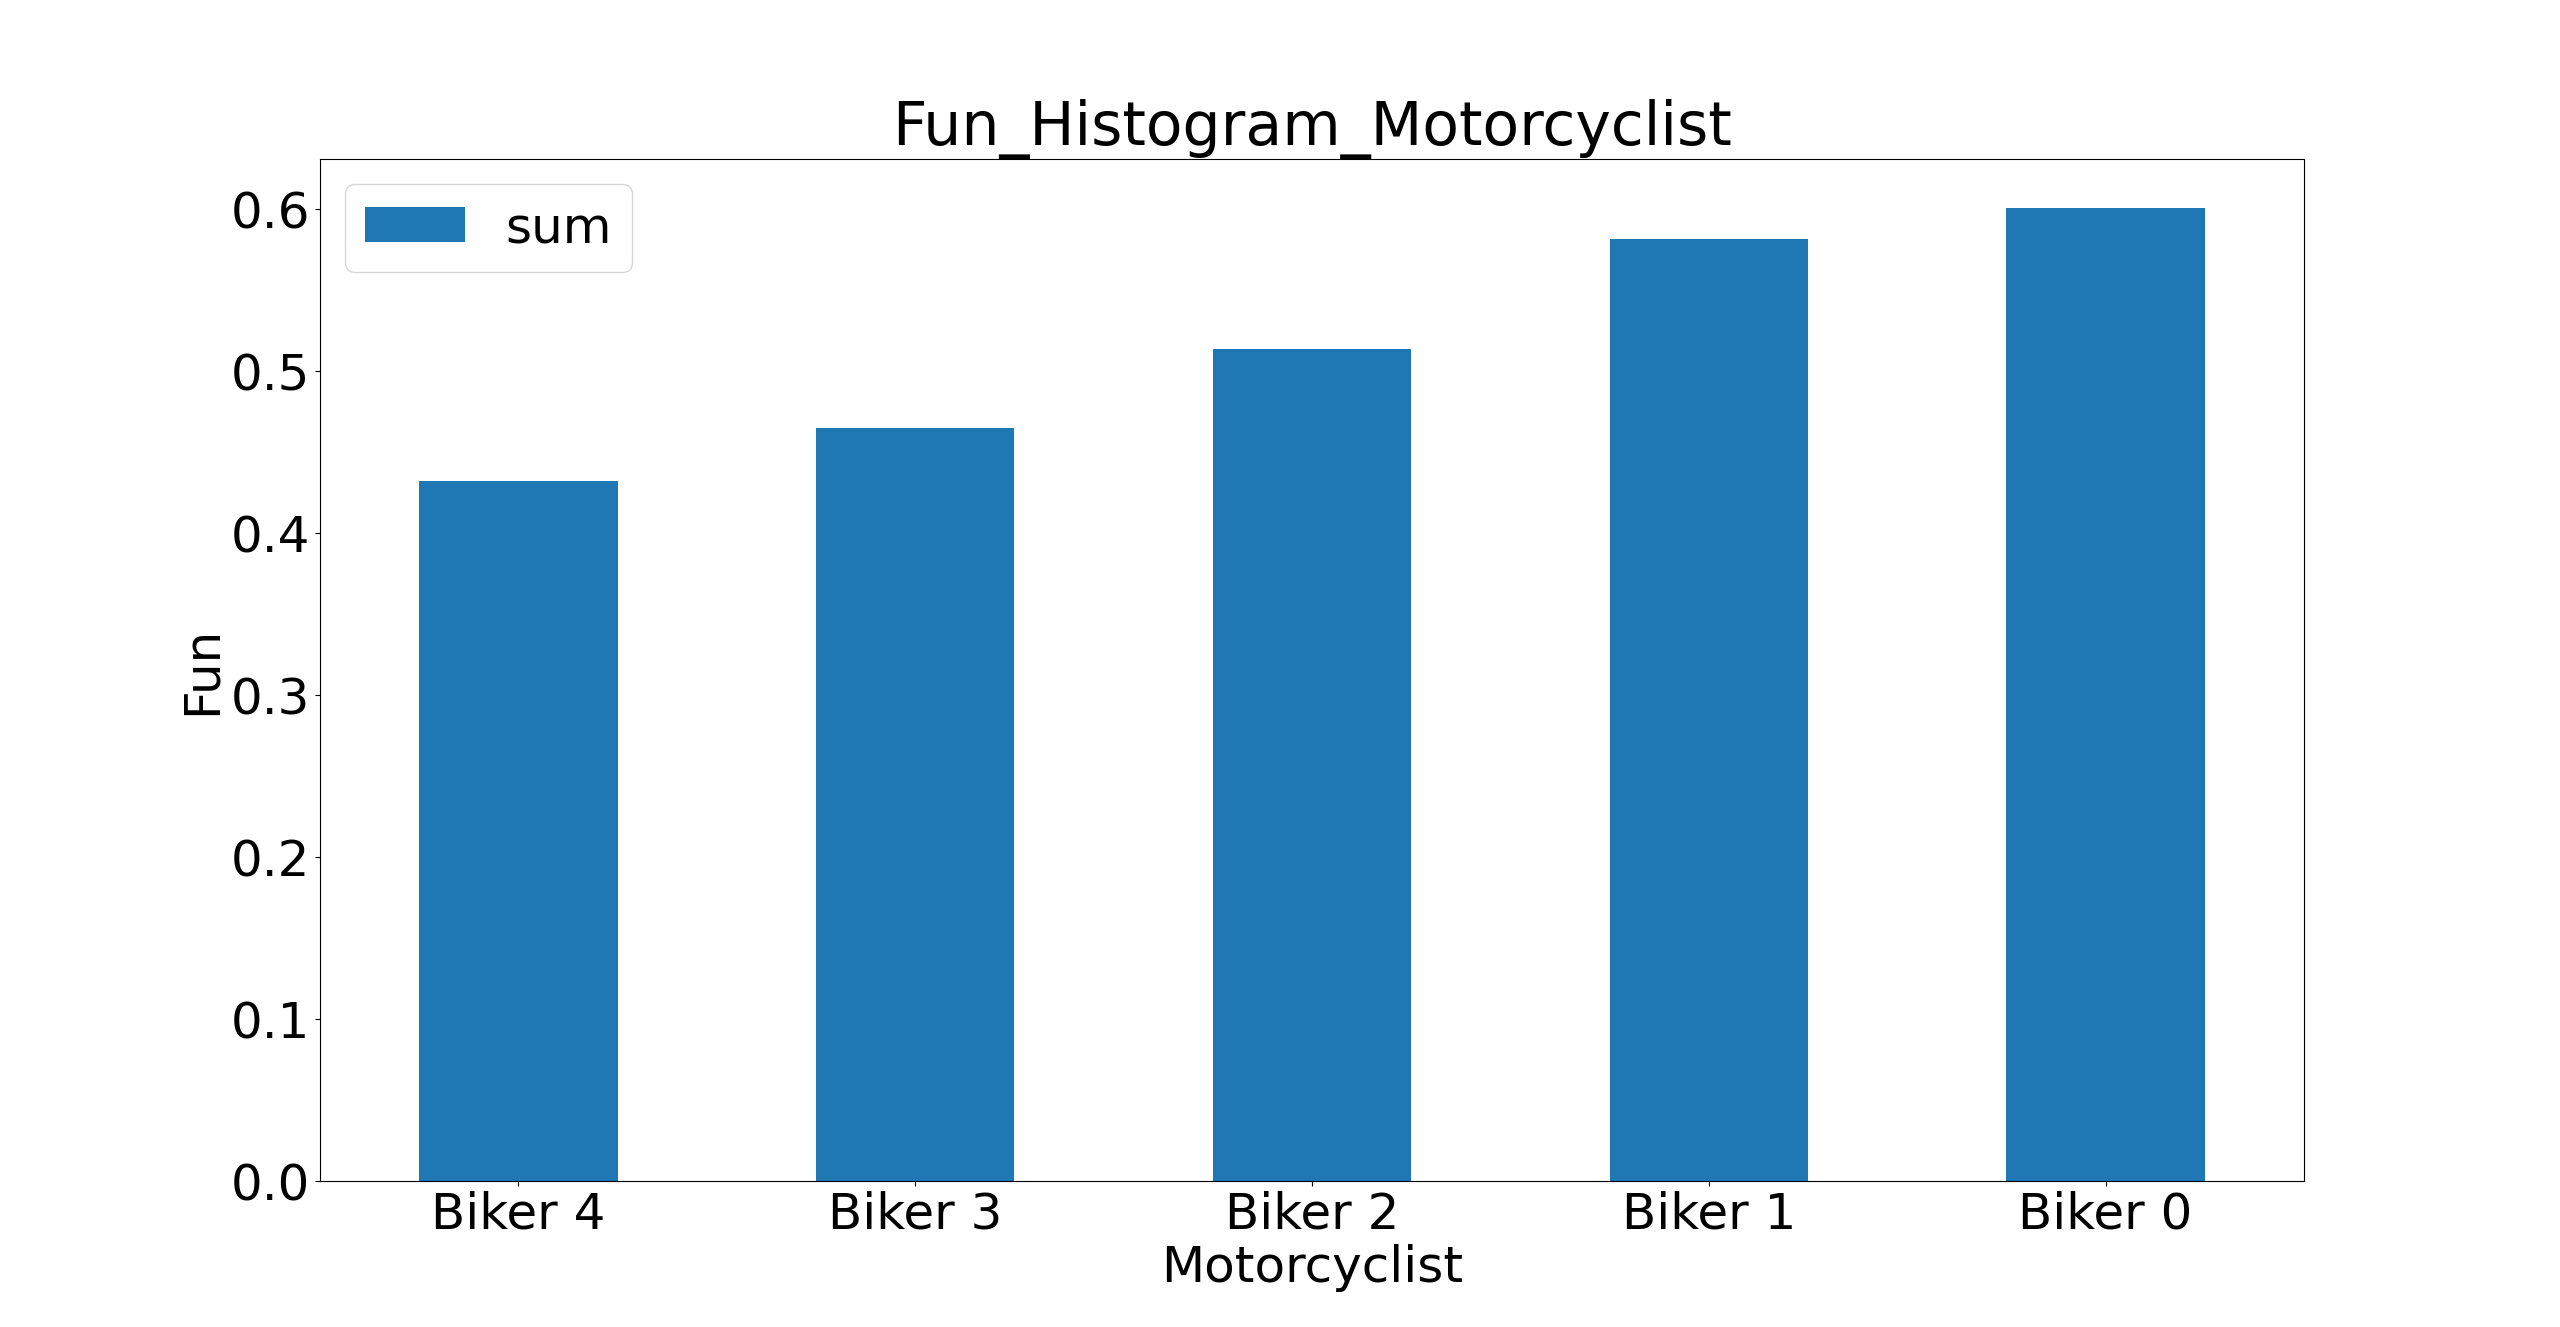
\includegraphics[width=\textwidth]{images/Allerheiligenstraße/Allerheiligenstrase_Fun_Histogram_congested.png}
         \caption{congested traffic}
     \end{subfigure}
        \caption{Fun-Distribution Histogram of five motorcyclists for Allerheiligenstraße}
        \label{fig:Allerheiligenstraße_fun_histogram}
\end{figure}

\begin{figure}
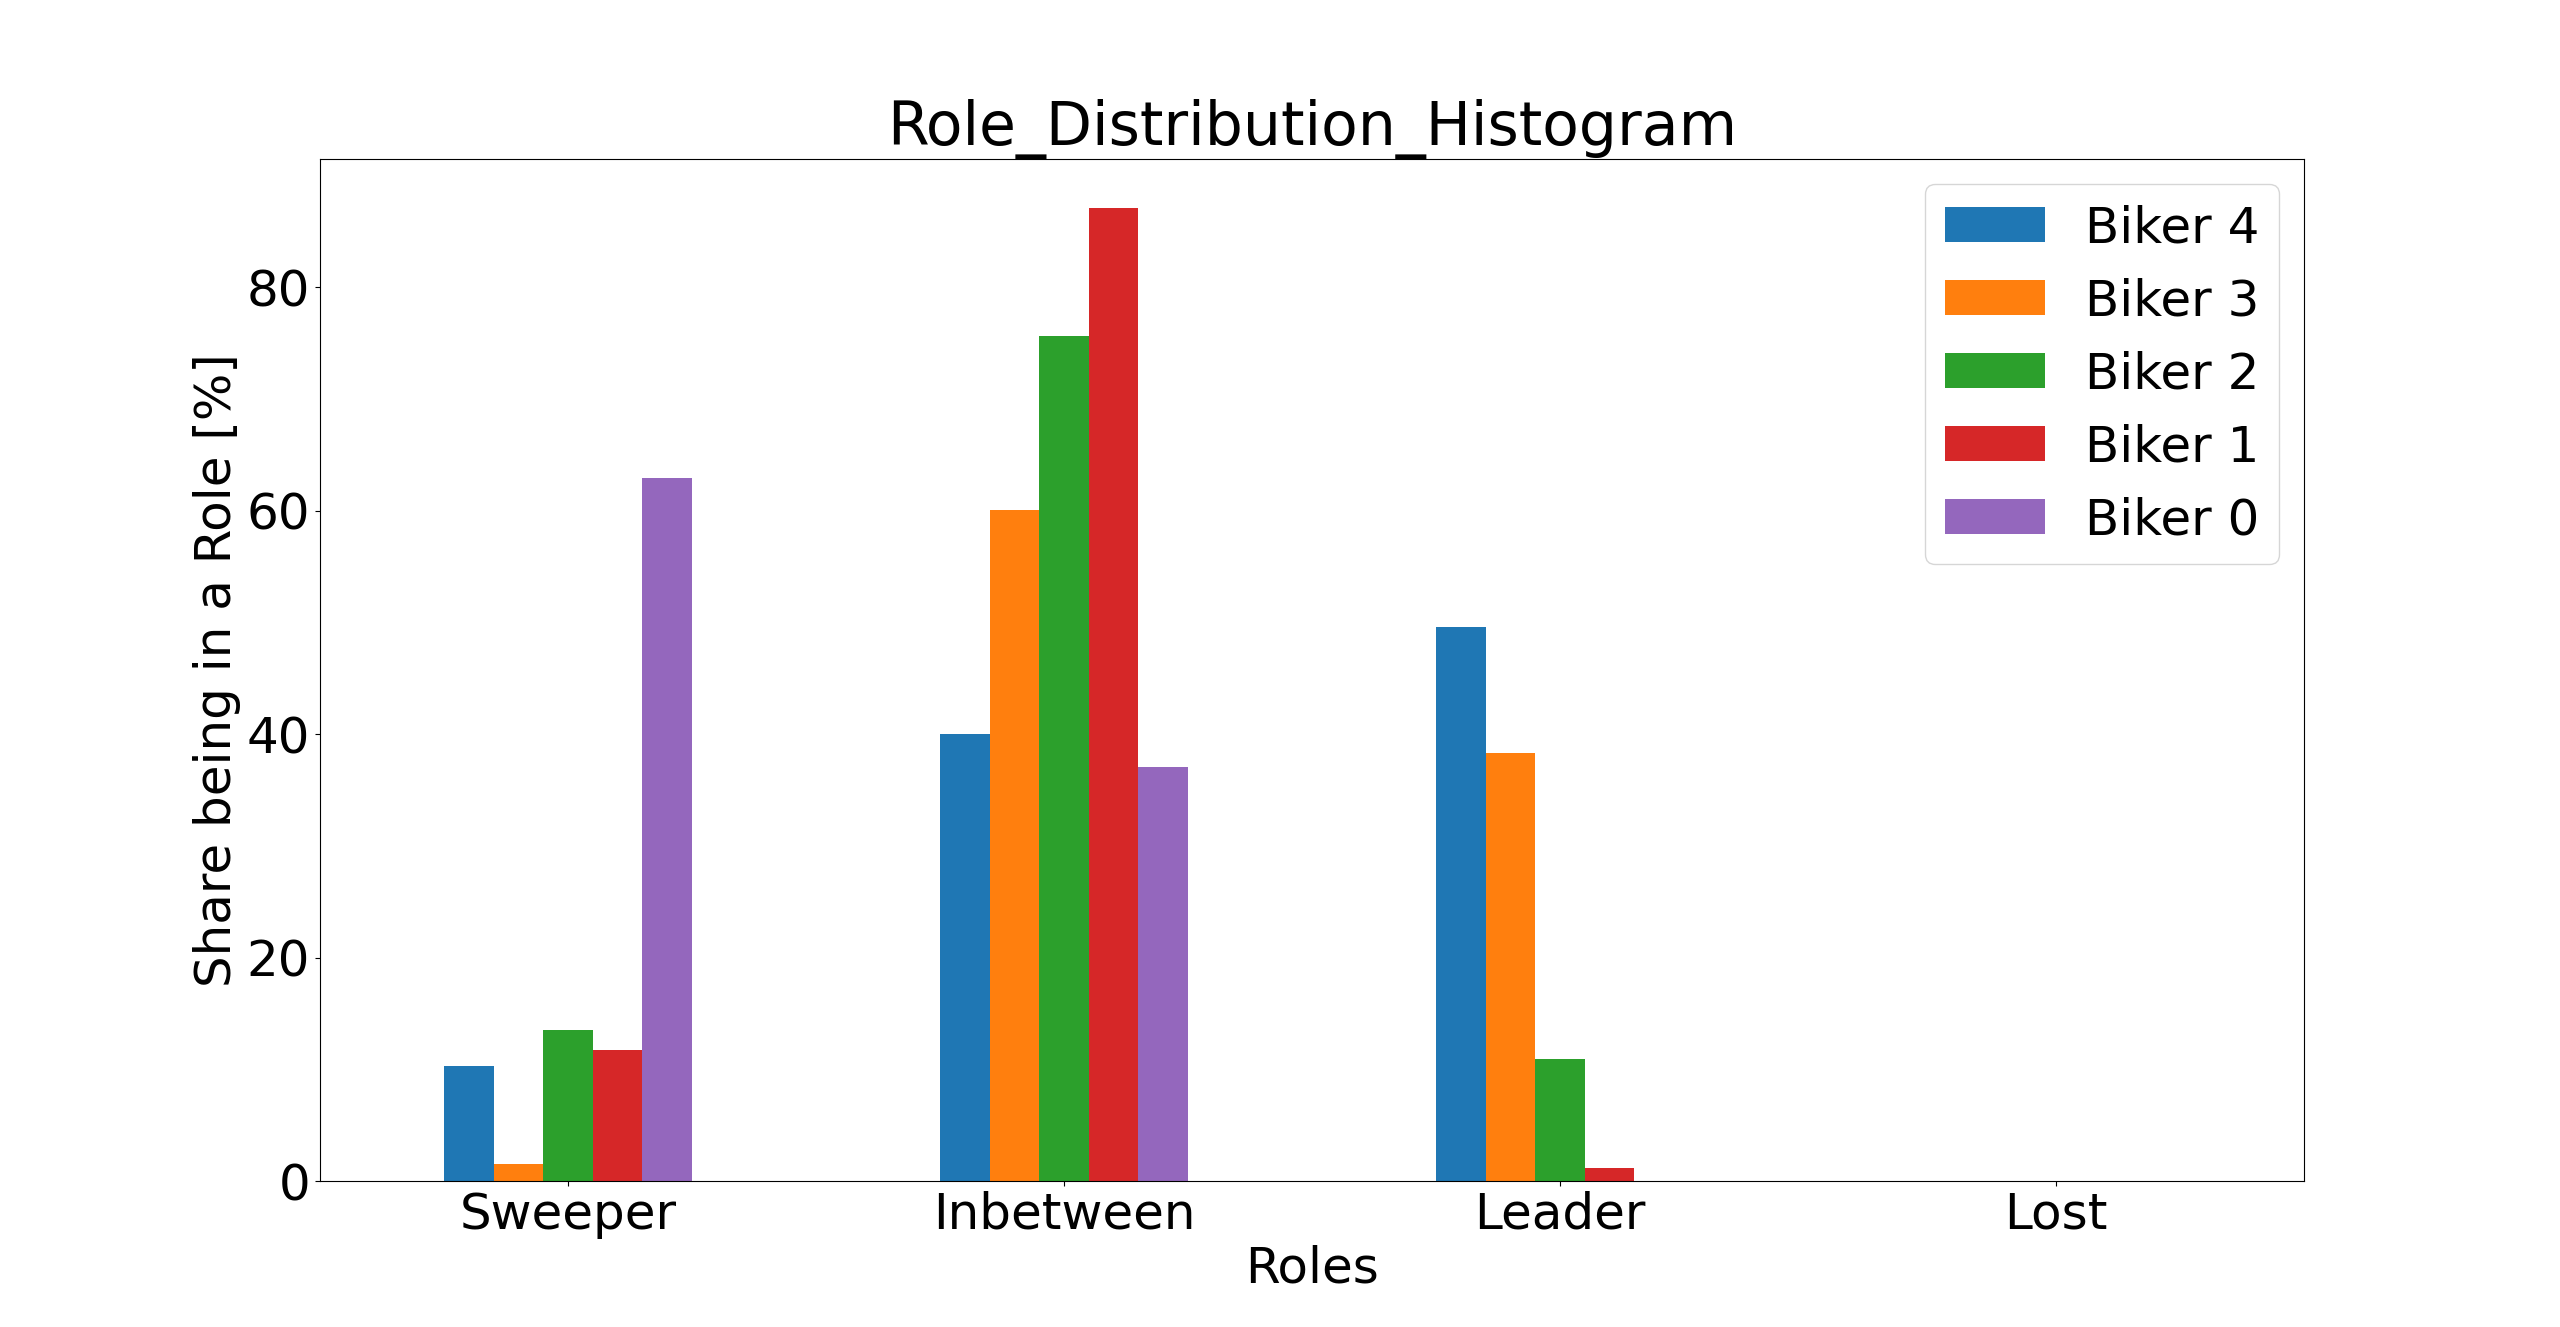
\includegraphics[width=1.0\linewidth]{images/Allerheiligenstraße/Allerheiligenstrase_Role_Distribution_Histogram_congested.png}
\caption{Role Distribution for Allerheiligenstraße in congested traffic}
\label{fig:Allerheiligenstraß_role_histogram}
\end{figure}

Figure \ref{fig:Allerheiligenstraß_lane_histogram} shows the percentage of time that a motorcyclist is on the right lane in congested traffic, which indicates that the platoon had to switch to the left lane due to perceived obstacles. Since the lane-changing rule is asymmetric, a lower percentage of time spent on the right lane suggests that more overtaking maneuvers were initiated due to perceived obstacles. Since only the leader can initiate an overtaking maneuver, differences in the percentage of time spent on the right lane indicate that the roles within the platoon may have changed over time. However, further research is necessary to establish a correlation between the roles and driving on the right lane. Additionally, it is surprising that the percentage is only around 80\%, given the street density of 3\%. Further Biker 3 shows an unexpectedly lower percentage of time spent on the right lane than the other bikers, which could be due to statistical error (since only 10 loops are performed). However, further research needs to be done to establish any possible correlations.\\


\begin{figure}
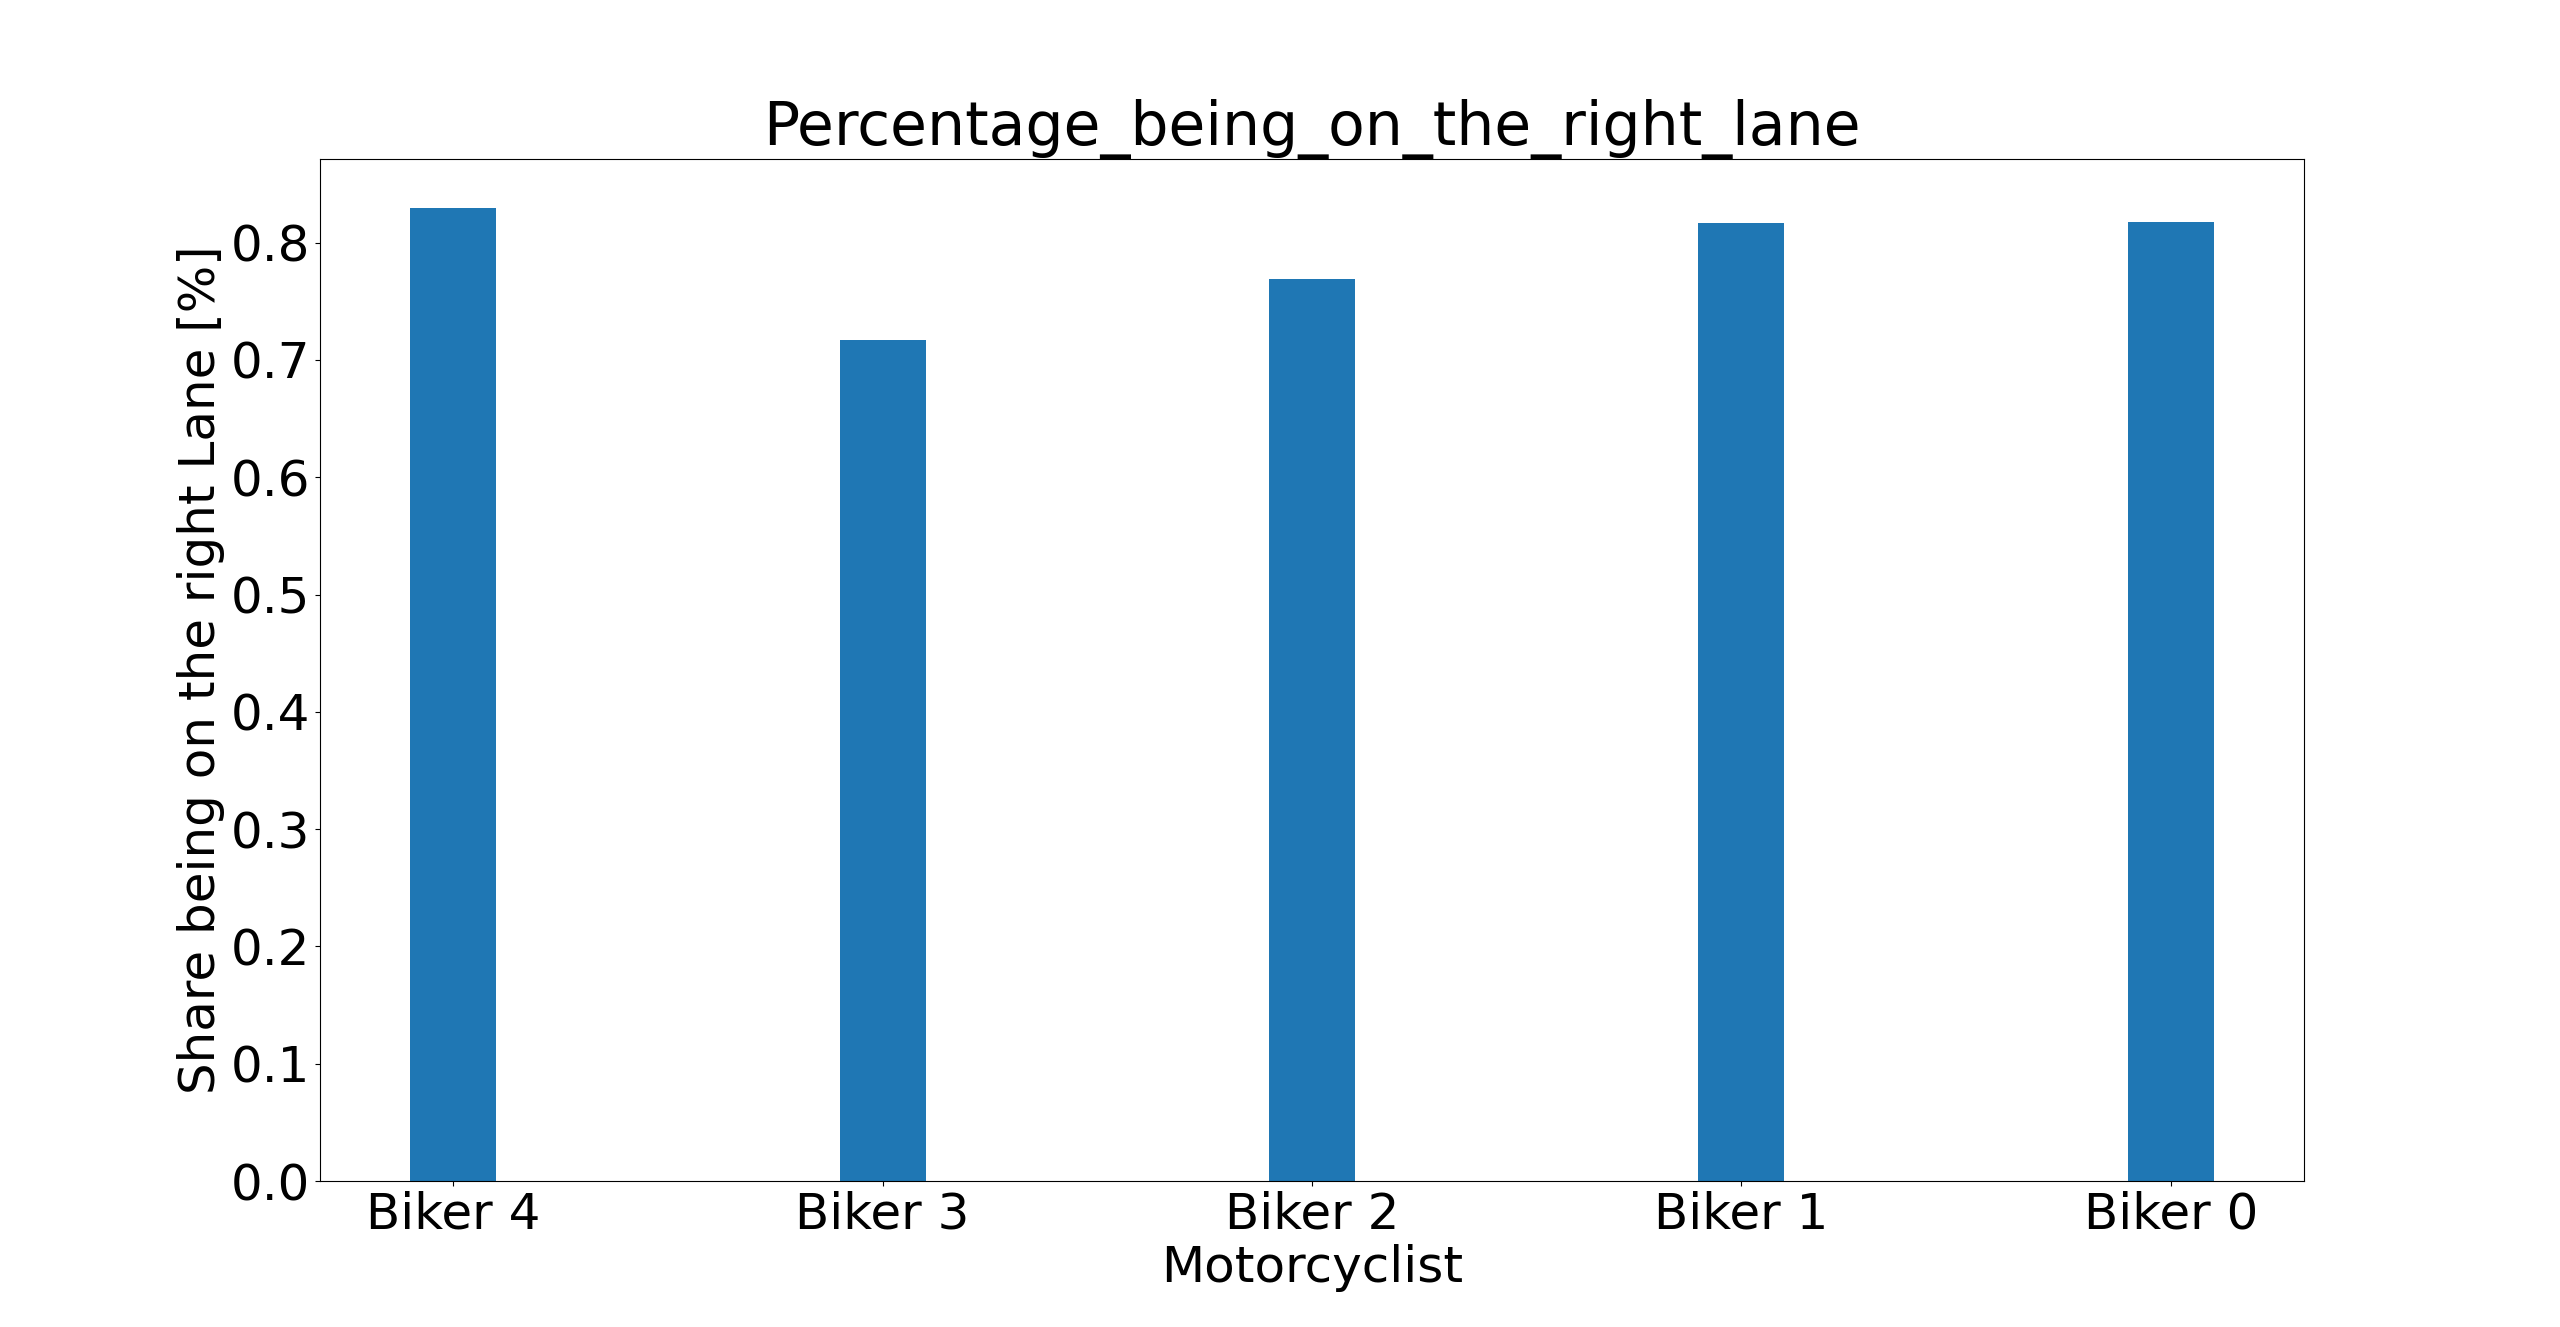
\includegraphics[width=1.0\linewidth]{images/Allerheiligenstraße/Allerheiligenstrase_Percentage_being_on_the_right_lane_congested.png}
\caption{Percentage bikers being on the right lane for Allerheiligenstraße in congested traffic}
\label{fig:Allerheiligenstraß_lane_histogram}
\end{figure}

Figure \ref{fig:Allerheiligenstraße_traveling} presents a mean velocity boxplot and the corresponding traveled distance for the five motorcyclists on a congested Allerheiligenstraße. The plot suggests that the platoon managed to stay together in a line, driving at the same velocity, with no noticeable abnormalities. The traveled distance diagram also demonstrates consistent behavior of the platoon, with each biker covering roughly the same distance over time. However, the deviation between each loop is significant, nearly 1000 tiles, indicating that the platoon may be getting split apart as the trip progresses.
As Biker 0 is positioned at the back of the platoon, their speed is likely to be more influenced by brakes in the front, leading to fewer outliers of higher speed and more outliers of lower speed compared to other bikers. This is a classic example of the bullwhip effect, where small variations velocity at the beginning of a chain can lead to larger and larger fluctuations further down the chain. The bullwhip effect can lead to inefficiencies in the platoon and decrease the overall throughput of the road, especially if the platoon is of significant size. As the bikers prioritize keeping a constant distance to the partner behind them, this effect can exacerbate the fluctuations in speed and distance between the bikers.\\

\begin{figure}
     \centering
     \begin{subfigure}[b]{1.0\textwidth}
         \centering
         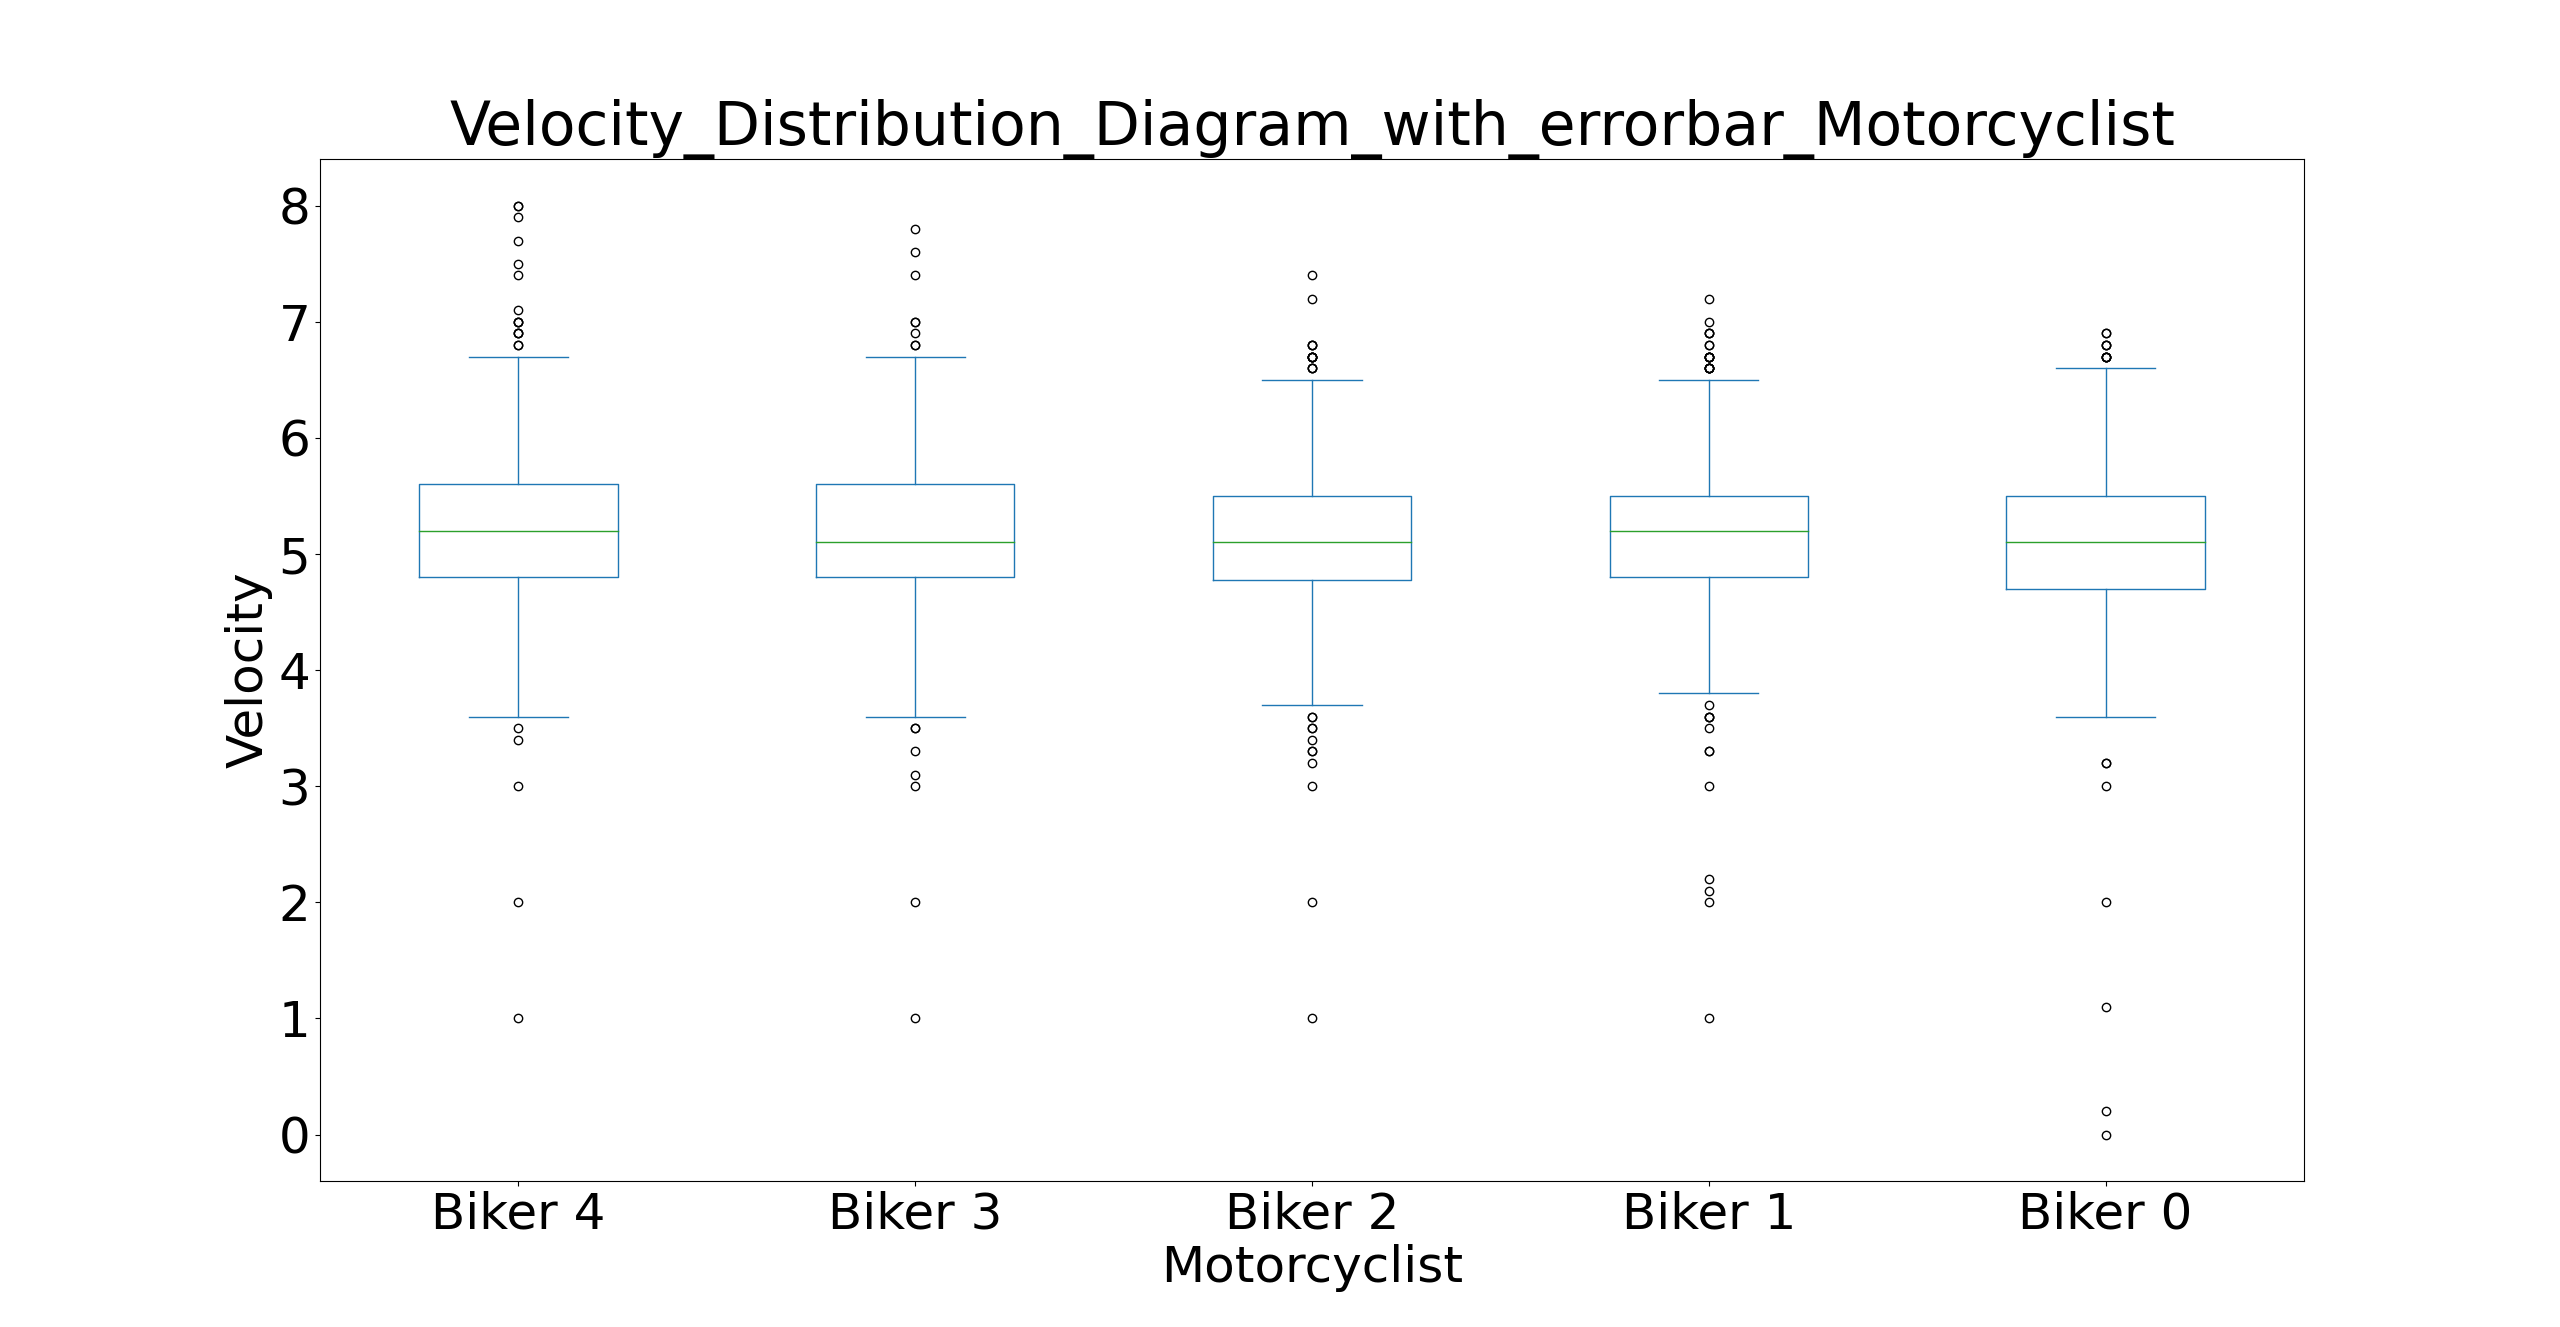
\includegraphics[width=\textwidth]{images/Allerheiligenstraße/Allerheiligenstrase_Velocity_Distribution_Diagram_with_errorbar_congested.png}
         \caption{Mean Velocity Boxplot}
     \end{subfigure}
     \hfill
     \begin{subfigure}[b]{1.0\textwidth}
         \centering
         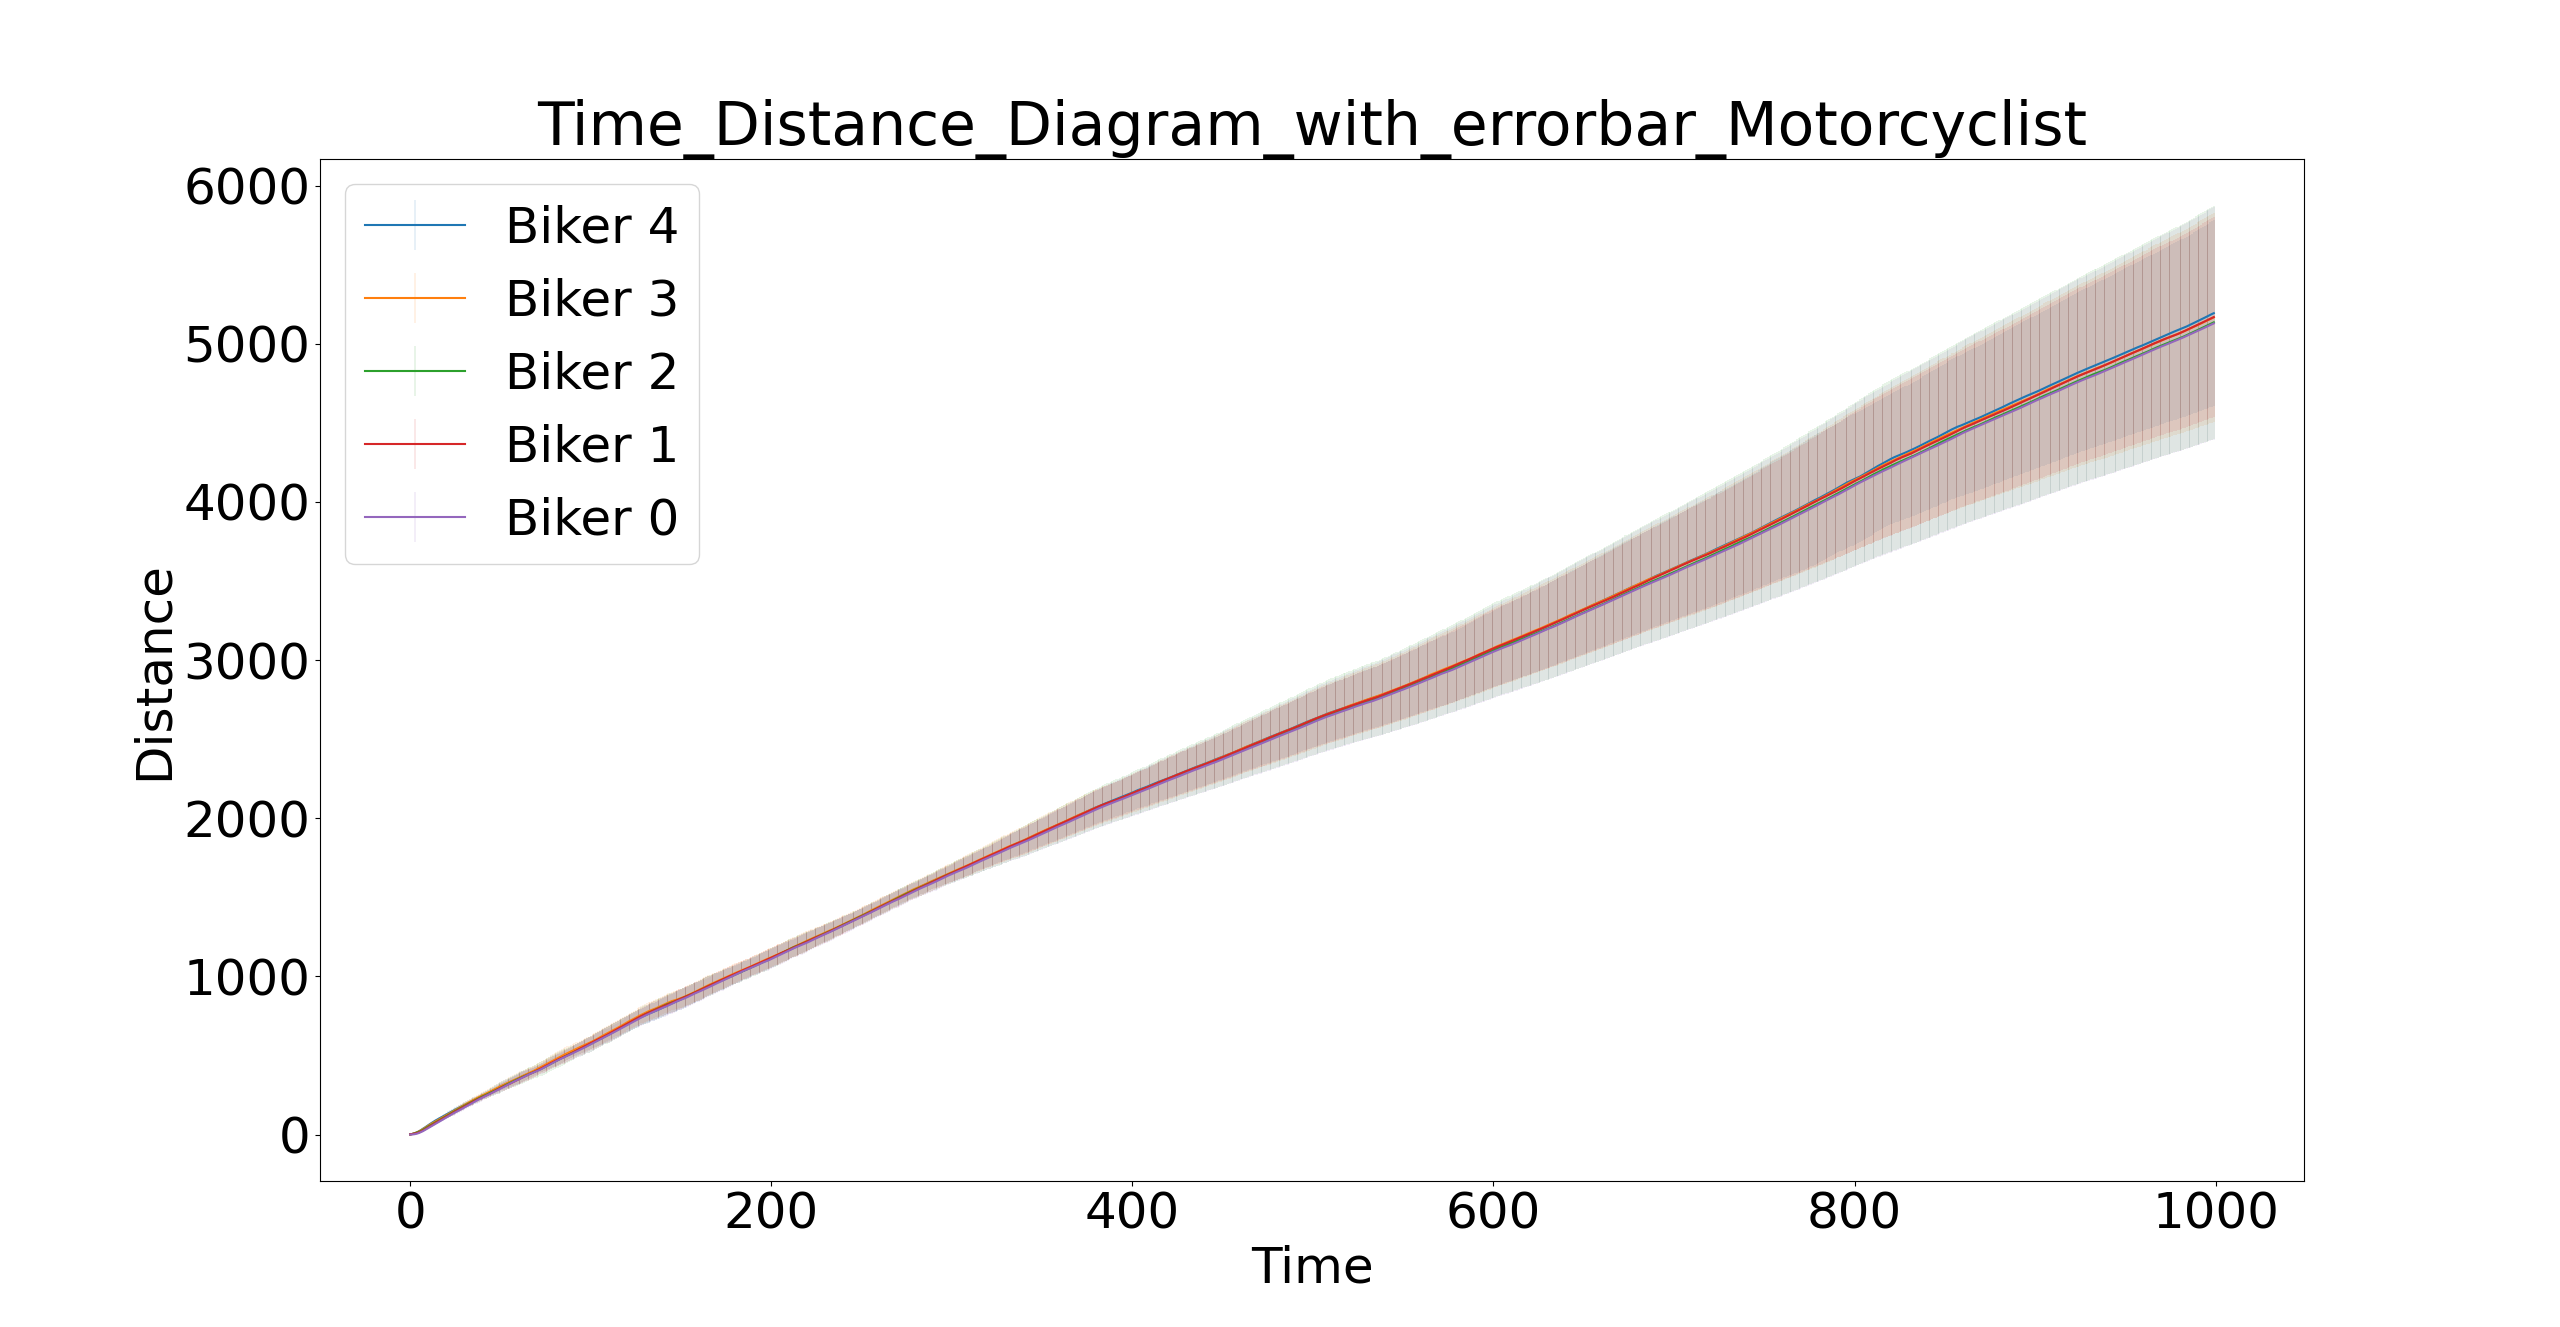
\includegraphics[width=\textwidth]{images/Allerheiligenstraße/Allerheiligenstrase_Time_Distance_Diagram_with_errorbar_congested.png}
         \caption{Traveled Distance Diagram}
     \end{subfigure}
        \caption{Mean Velocity Boxplot and corresponding Traveled Distance Diagram for five bikers on a congested Allerheiligenstraße}
        \label{fig:Allerheiligenstraße_traveling}
\end{figure}

Figure \ref{fig:Allerheiligenstraße_distance_partner} shows the mean distance between the motorcyclists both altogether and separately within a platoon on a free and congested Allerheiligenstraße. On a free traffic road, there are strong fluctuations in the middle of the trip, which overlap with the actual curvature of Allerheiligenstraße, as the platoon tries to maintain a constant distance of 5 tiles between each other. These fluctuations have a direct impact on the fun-distribution diagram in figure \ref{fig:Allerheiligenstraße_fun_distribution}, as seen earlier. In congested traffic, the interpretation is more difficult. The increase in the spread of the distance between each other over time can be expected, as the traveled distance seen in figure \ref{fig:Allerheiligenstraße_traveling} also shows an increased spread over time. However, when comparing the $distance\_to\_partner$ distributions of the free and congested roads in figure \ref{fig:Allerheiligenstraße_distance_partner}, no correlation with road curvature is found, suggesting that road curvature has no effect on the break-up of the platoon. The combination of the higher variance in the distance to partners and the spread in the traveled distance could result in some motorcyclists falling far behind, leading to a higher variance at the end. This observation is also supported by Figure \ref{fig:Allerheiligenstraß_distance_partner_separate}, which suggests that the motorcyclists got separated during the process. This separation could be caused by cars getting stuck next to each other on the left and right lanes, which might explain why groups can get separated. During the coding phase, this possibility was not taken into account.\\

\begin{figure}
     \centering
     \begin{subfigure}[b]{1.0\textwidth}
         \centering
         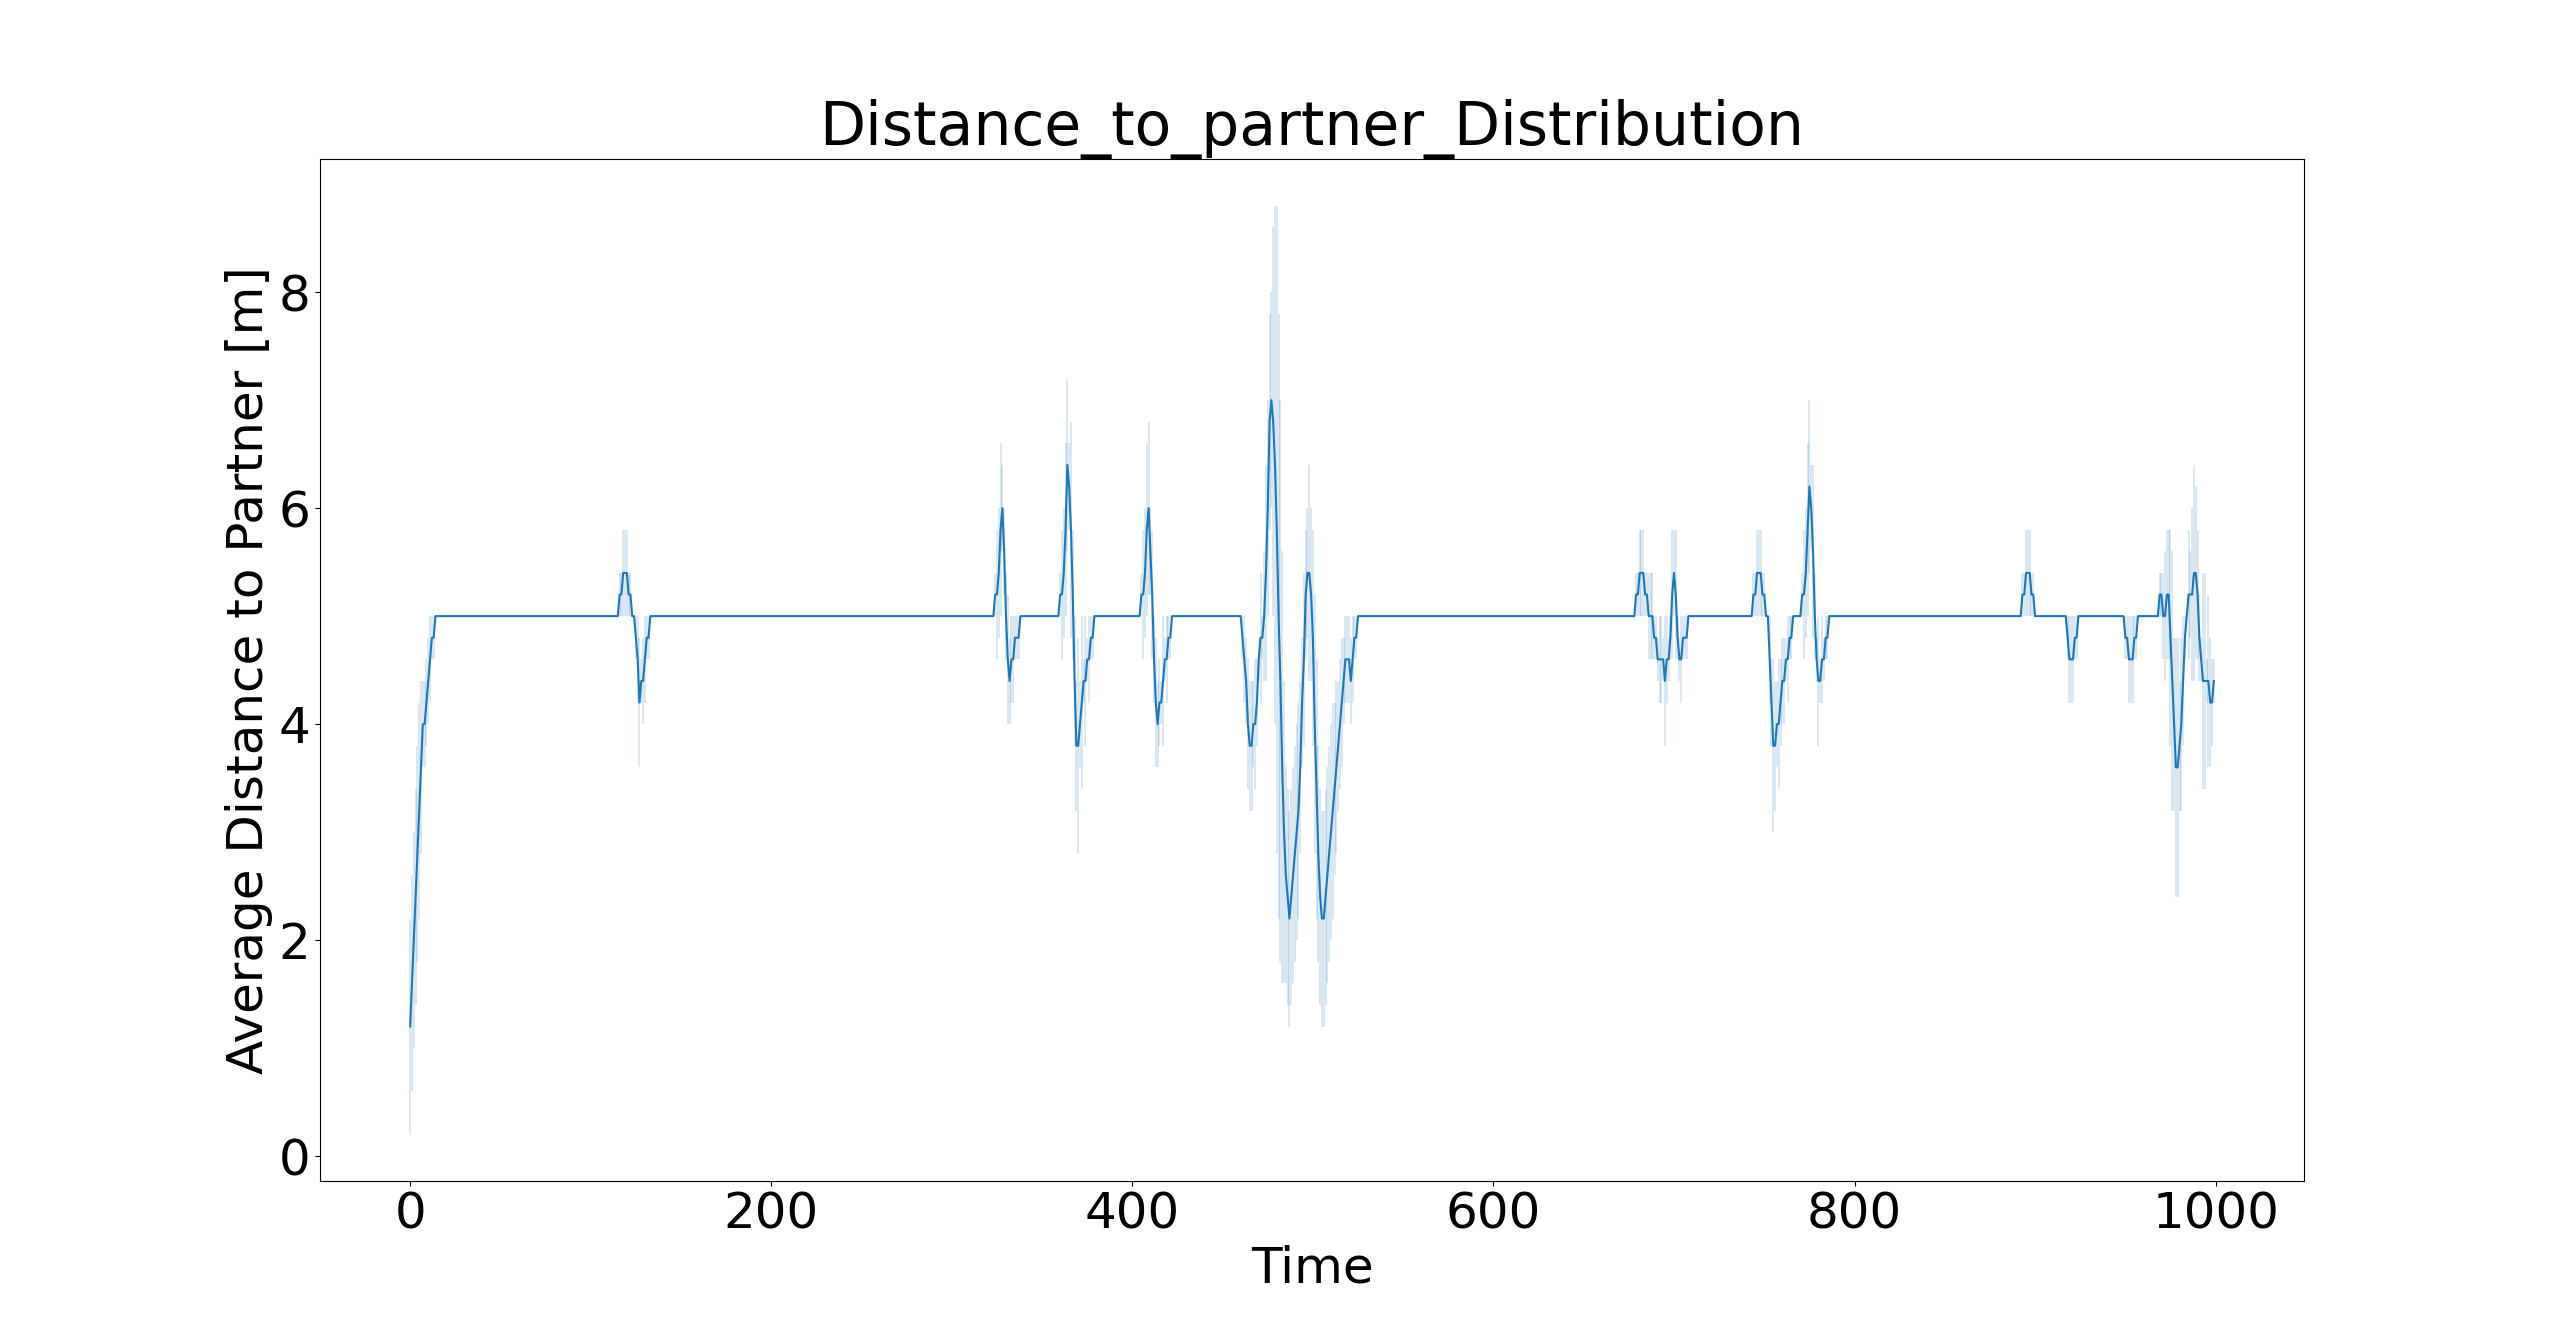
\includegraphics[width=\textwidth]{images/Allerheiligenstraße/Allerheiligenstrase_AVG_Distance_to_partner_distribution_free.png}
         \caption{Average distance to partner over time for all bikers in free traffic}
     \end{subfigure}
     \hfill
     \begin{subfigure}[b]{1.0\textwidth}
         \centering
         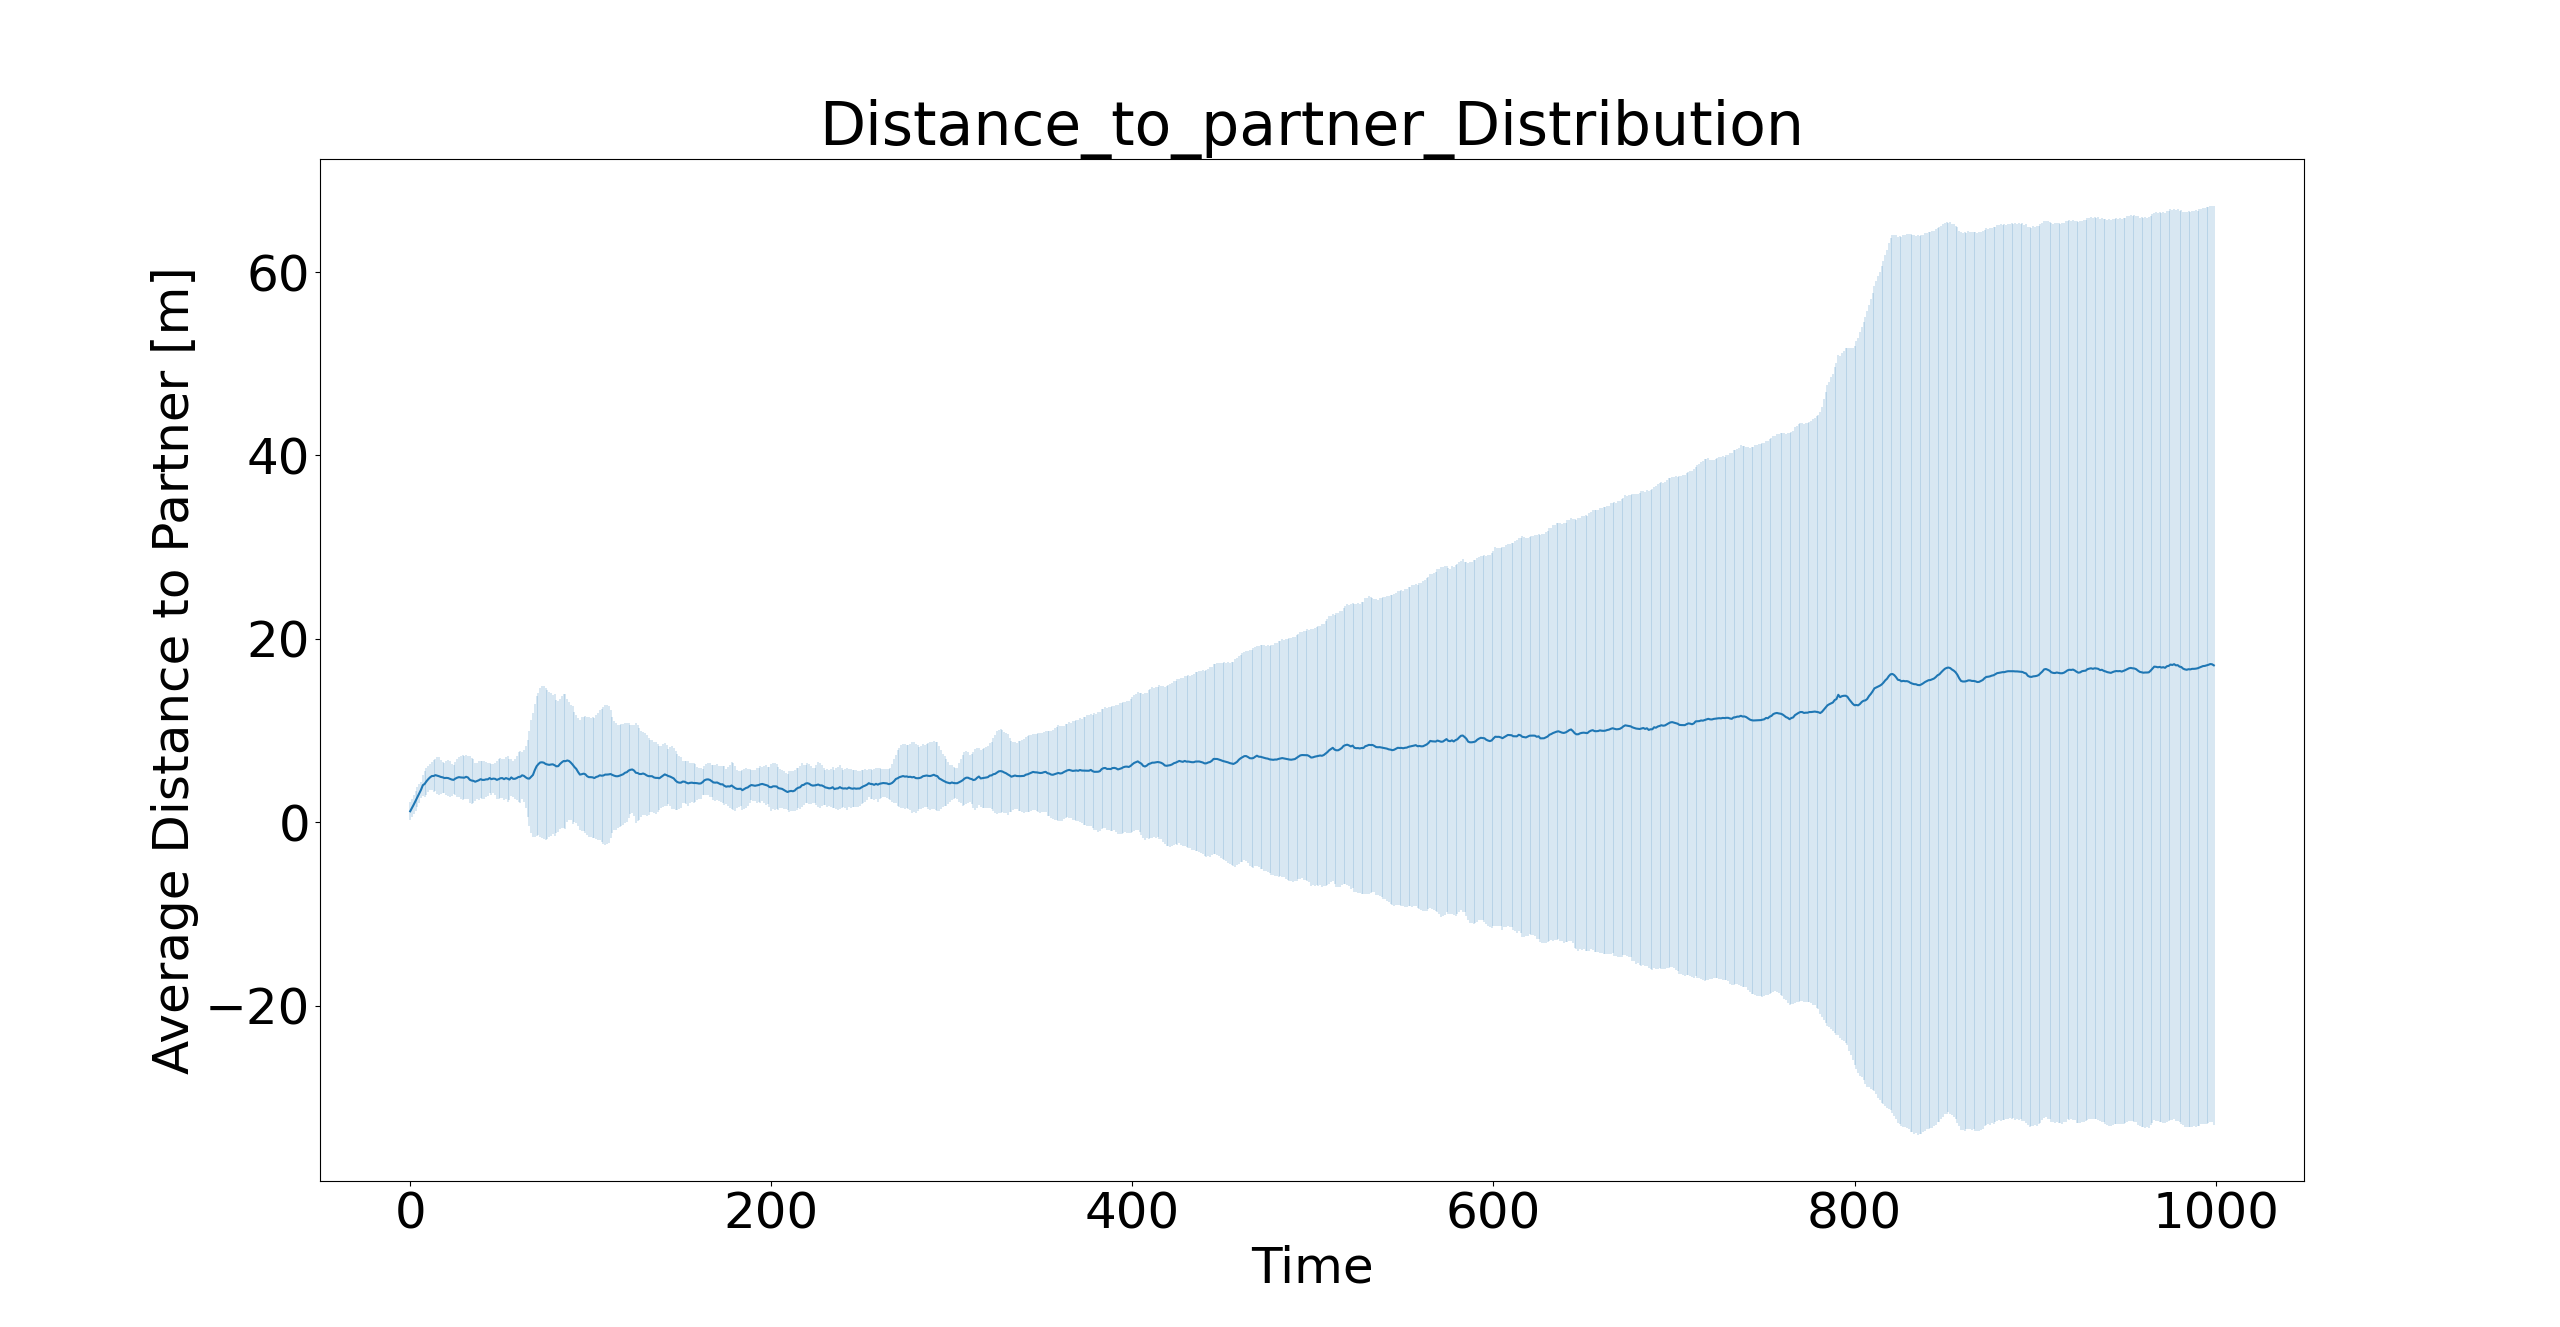
\includegraphics[width=\textwidth]{images/Allerheiligenstraße/Allerheiligenstrase_AVG_Distance_to_partner_distribution_congested.png}
         \caption{Average distance to partner over time for all bikers in congested traffic}
     \end{subfigure}
        \caption{Average distance to the partner of a motorcyclist in free and congested Allerheiligenstraße}
        \label{fig:Allerheiligenstraße_distance_partner}
\end{figure}

\begin{figure}
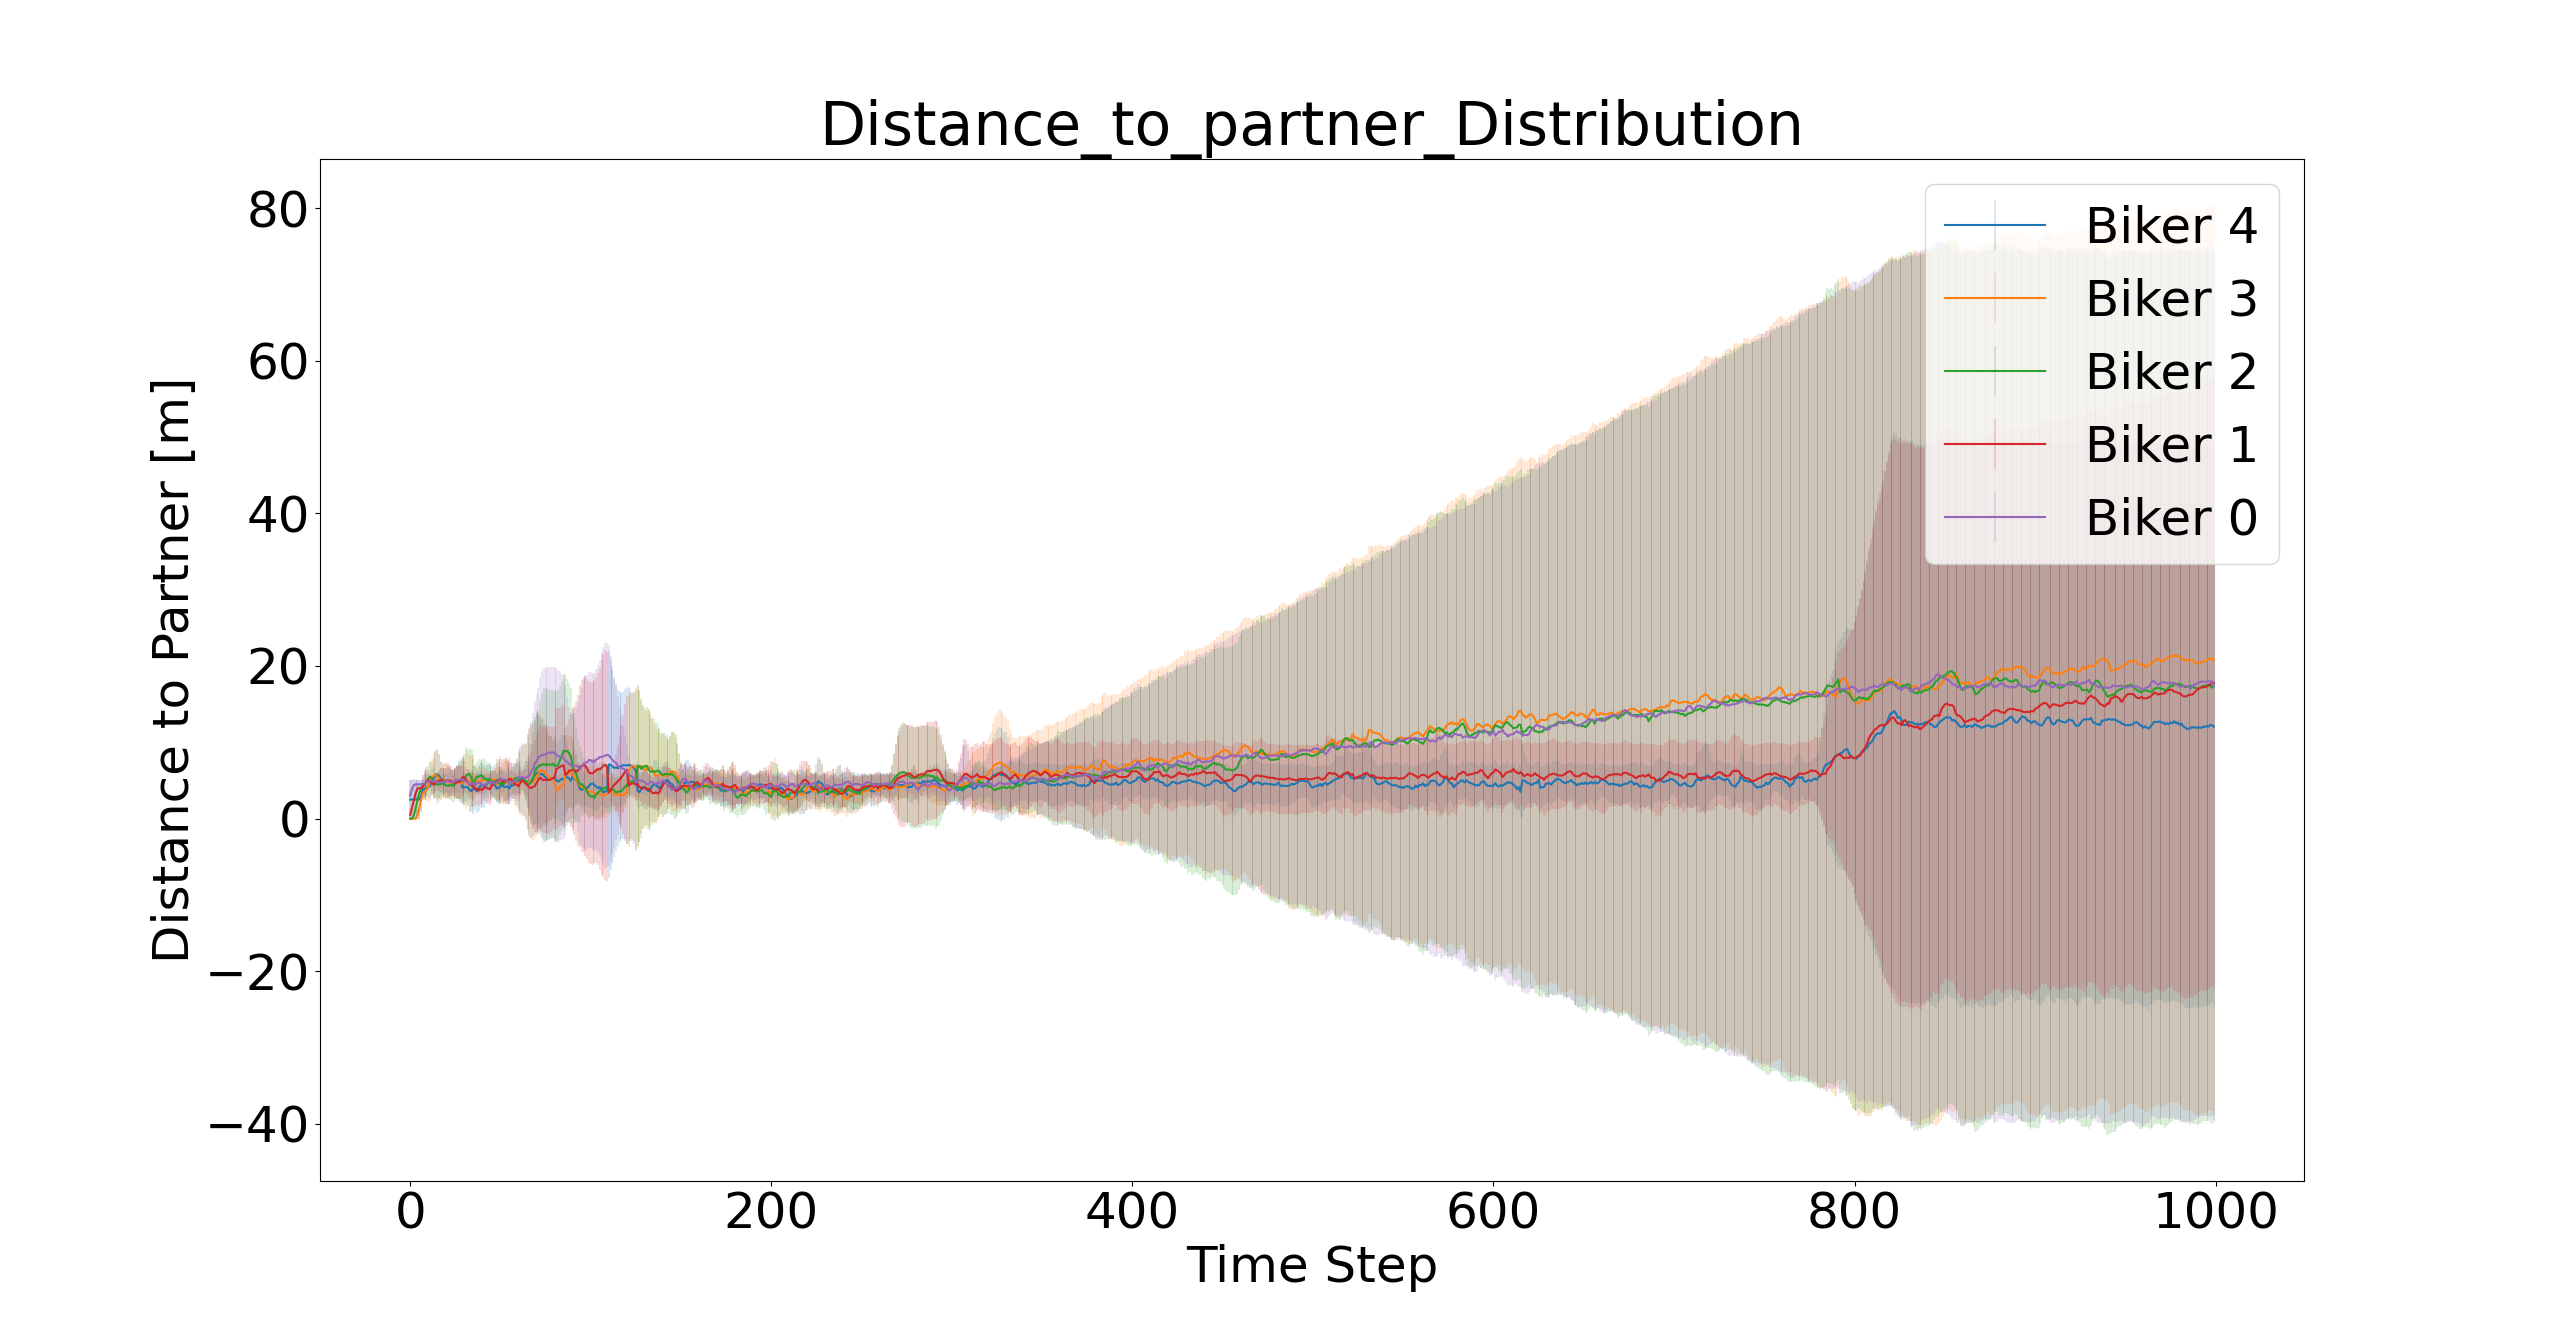
\includegraphics[width=1.0\linewidth]{images/Allerheiligenstraße/Allerheiligenstrase_Distance_to_partner_distribution_congested.png}
\caption{Average distance to partner over time in congested traffic}
\label{fig:Allerheiligenstraß_distance_partner_separate}
\end{figure}

The results for the other roads show similar behavior and no major anomalies were found. The plots can be found in the Appendix \ref{chapter:Appendix: Appendix: Additional Simulation Results}.


\section{Ranking of the Streets}
\label{Ranking of the Streets}
This section examines whether the use of the fun metric to rate roads correlates with overall curvature, as it might be expected that a more curvy road would be more fun to drive than a less curvy one.  
The simulation results for the seven selected roads are summarized in table \ref{tab:ranking}. The \textit{[curvature]} column shows the total curvature of each road, while the \textit{[sum fun free]} and \textit{[sum fun congested]} columns show the total fun values accumulated by all bikers during the ten loops for free and congested roads respectively. The \textit{[time steps]} column shows the number of time-steps taken by the platoon during a loop. The values for curvature and fun are then normalized by time-step, which can be found in the columns \textit{[curvature per time step]}, \textit{[sum fun per time step free]} and \textit{[sum fun per time step congested]}. The ranking for each metric is given in the columns \textit{[rank curvature]}, \textit{[rank fun free]} and \textit{[rank fun congested]}, from highest to lowest.\\

\begin{landscape}
\begin{table}
\centering
\begin{tabular}{|p{3.5cm}|p{1.5cm}|p{1.5cm}|p{1.5cm}|p{1.5cm}|p{1.5cm}|p{1.5cm}|p{1.5cm}|p{1cm}|p{1cm}|p{1cm}|}
\toprule
\textit{street} & \textit{curvature} & \textit{sum fun free} & \textit{sum fun congested} & \textit{time steps} & \textit{curvature per time step} & \textit{sum fun per time step free} & \textit{sum fun per time step congested} & \textit{rank curvature} & \textit{rank fun free} & \textit{rank fun congested} \\
\midrule
Großherzog-Friedrich-Luisen-Straße  & 12106 & 43692 & 27951 & 820   & 15 & 53 & 34 & 1 & 2 & 1 \\
Wildschapbachstraße                 & 9488  & 40201 & 21185 & 745   & 13 & 54 & 28 & 2 & 1 & 2 \\
Allerheiligenstraße                 & 12168 & 52118 & 25930 & 1000  & 12 & 52 & 26 & 3 & 4 & 3 \\
Nordracher Straße                   & 6290  & 33966 & 16805 & 650   & 10 & 52 & 26 & 4 & 3 & 4 \\
Kaltenbronner Straße                & 6917  & 45057 & 16882 & 900   & 8  & 50 & 19 & 5 & 5 & 7 \\
Rippoldsauer Straße                 & 11055 & 67102 & 28825 & 1500  & 7  & 45 & 19 & 6 & 7 & 6 \\
Sandstraße                          & 8439  & 58670 & 24366 & 1190  & 7  & 49 & 20 & 7 & 6 & 5 \\
\bottomrule
\end{tabular}
\caption{Ranking of the streets according to curvature and fun values gathered}
\label{tab:ranking}
\end{table}
\end{landscape}

To measure the correlation between two variables and identify its statistical significance, the Spearman's rank correlation coefficient was used. The Spearman's rank correlation coefficient is a nonparametric measure and assesses the strength and direction of monotonic relationships between ranked variables. The formula for its calculation is as follows\footnote{see: https://en.wikipedia.org/wiki/Spearman's\_rank\_correlation\_coefficient, accessed on February 20, 2023}:

\begin{align}
s &= 1 - \frac{6 \sum_{i=1}^n (R_i - S_i)^2}{n(n^2 - 1)}
\label{eq:spearman}
\end{align}

In this equation, n represents the number of observations, $R_i$ and $S_i$ represent the ranks of the i'th observation in each of the two variables being compared. The Spearman rank correlation coefficient ranges from -1 (perfect negative correlation) to +1 (perfect positive correlation). \\

The Spearman's rank coefficient values between the rankings obtained from the simulation are presented in table \ref{tab:spearman_results}. The statistical significance of these coefficients was determined by comparing them with the Spearman rank correlation table of critical values in table \ref{fig:spearmancritical}, this table is suitable for smaller samples\footnote{see: https://real-statistics.com/correlation/spearmans-rank-correlation/spearmans-rank-correlation-detailed/, 20.02.2023}. Based on the Spearman's rank coefficients, it is evident that there is a positive correlation between the rankings obtained from the simulation. All coefficients show a correlation of at least 0.82, which is above the critical value of 0.714 for a significance level of 5\% and a sample size of seven. Therefore the null hypothesis can be rejected at a 5\% significance level according to the two-tail test.
This suggests that the simulation setup can support the hypothesis that the more twisty the road, the more fun it is for a platoon to drive. Road congestion has no effect on the results. However, as the results are not statistically significant at the 1\% level and the sample size is relatively small, as well as the lack of an actual survey, the conclusion should be treated with caution.



\begin{table}
    \centering
    \begin{tabular}{|c|c|} 
        \hline
        Correlation & Coefficient \\ \hline
        $s_{rank\,curvature; rank\,fun\,free}$ & 0.893 \\ 
        $s_{rank\,curvature; rank\,fun\,congested}$ & 0.857 \\
        $s_{rank\,fun\,free; rank\,fun\,congested}$ & 0.821 \\
        \hline
    \end{tabular}
    \caption{Spearman correlation coefficients between different ranks}
    \label{tab:spearman_results}
\end{table}

\begin{figure}
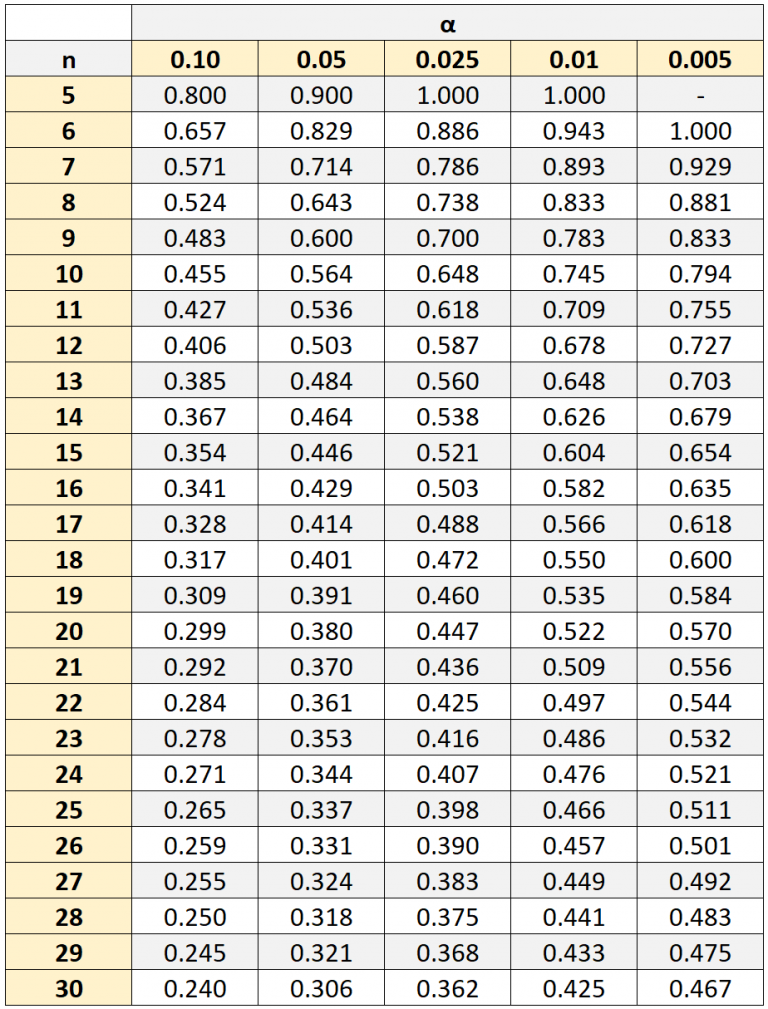
\includegraphics[width=1.0\linewidth]{images/spearmancritical.png}
\caption{Critical Values of the Spearman’s Ranked Correlation Coefficient, source: www.statology.org/spearman-rank-correlation-google-sheets/, 20.02.2023}
\label{fig:spearmancritical}
\end{figure}



